% AI6127 Group 6 project report. Build: latexmk -pdf main.tex (see README.md in this folder).
\documentclass[11pt]{article}
\PassOptionsToPackage{hyphens}{url}

% "preprint": non-anonymous, with page numbers. Switch to "final" to drop the page numbers.
\usepackage[preprint]{acl}

\usepackage{times}
\usepackage{latexsym}
\usepackage[T1]{fontenc}
\usepackage[utf8]{inputenc}
\usepackage{microtype}
\usepackage{inconsolata}
\usepackage{graphicx}
\usepackage{booktabs}
\usepackage{placeins}
\usepackage{multirow}
\usepackage{array}
\usepackage{xcolor}
\usepackage{tikz}
\usetikzlibrary{arrows.meta,positioning,shapes.geometric,fit,calc}
\usepackage{pgfplots}
\pgfplotsset{compat=newest}

% ---------------------------------------------------------------------------------------------
% Fill in once; everything below reads these macros.
% ---------------------------------------------------------------------------------------------
\newcommand{\groupno}{6}
\newcommand{\memberA}{Member One}   \newcommand{\matricA}{G2XXXXXXA} \newcommand{\mailA}{member1@e.ntu.edu.sg}
\newcommand{\memberB}{Member Two}   \newcommand{\matricB}{G2XXXXXXB} \newcommand{\mailB}{member2@e.ntu.edu.sg}
\newcommand{\memberC}{Member Three} \newcommand{\matricC}{G2XXXXXXC} \newcommand{\mailC}{member3@e.ntu.edu.sg}
\newcommand{\memberD}{Member Four}  \newcommand{\matricD}{G2XXXXXXD} \newcommand{\mailD}{member4@e.ntu.edu.sg}
\newcommand{\memberE}{Member Five}  \newcommand{\matricE}{G2XXXXXXE} \newcommand{\mailE}{member5@e.ntu.edu.sg}
\newcommand{\memberF}{Member Six}   \newcommand{\matricF}{G2XXXXXXF} \newcommand{\mailF}{member6@e.ntu.edu.sg}
\newcommand{\datalink}{\url{https://drive.google.com/file/d/1k0vG2eQaOc13oEJcvT5vQMuVagxhZR1L/view?usp=sharing}}
\newcommand{\codelink}{\url{https://github.com/AY26-NLP-Group-6-Project/AY26-NLP-Group-Project}}
\newcommand{\sheetlink}{\url{https://docs.google.com/spreadsheets/d/176A5URtreDoXT9JHUQ1ykacDJudnrlmvuIhMU-e2_pI/edit?usp=sharing}}
\newcommand{\chatmodel}{\texttt{gpt-5.6-luna}}
\newcommand{\embmodel}{\texttt{text-embedding-3-small}}
\newcommand{\reranker}{\texttt{ms-marco-MiniLM-L-6-v2}}
\newcommand{\pending}{\textbf{[Pending Result]}}
% ----------------------------------------------------------------------------

\newcommand{\cond}[1]{\texttt{#1}}
% run names, file names and paths: typewriter, but allowed to break after / - _ .
\newcommand{\run}[1]{\nolinkurl{#1}}
\newcommand{\file}[1]{\nolinkurl{#1}}
\newcommand{\kappaval}{$\kappa$}
\newcolumntype{L}[1]{>{\raggedright\arraybackslash}p{#1}}
\makeatletter
\g@addto@macro\UrlBreaks{\do\_}
\makeatother
\Urlmuskip=0mu
% avoid stretched vertical gaps between paragraphs and around headings
\raggedbottom

\setlength\titlebox{7.5cm}

\title{Greenwash-RAG: Evidence-Grounded, Cross-Year Tracking of\\Sustainability Claims in SGX Reports\\
  {\large AI6127 Group Project Report, Group \groupno}}

\author{%
  \memberA \\ \matricA \\ \texttt{\mailA} \And
  \memberB \\ \matricB \\ \texttt{\mailB} \And
  \memberC \\ \matricC \\ \texttt{\mailC} \AND
  \memberD \\ \matricD \\ \texttt{\mailD} \And
  \memberE \\ \matricE \\ \texttt{\mailE} \And
  \memberF \\ \matricF \\ \texttt{\mailF} \\
}

\begin{document}
\maketitle

\begin{abstract}
Analysts reading sustainability reports want to know whether a company's dated commitments were kept, and where the evidence is. We build Greenwash-RAG, a retrieval-augmented system over 240 sustainability reports of 56 SGX-listed issuers (2020--2025, 3.5\,M words, 108,376 statement chunks) that answers with page-cited evidence through a Streamlit interface. A hybrid retriever (BM25 and dense retrieval with reciprocal rank fusion, cross-encoder re-ranking and company/year filters) reaches the best nDCG@10 on pooled, model-graded judgements (0.80 against 0.71 for BM25 alone), and a temporal claim graph returns precise but sparse cross-year evidence at a tenth of its latency. \textbf{RQ1} labels a sentence's sustainability action under the A3CG scheme on 1,000 self-annotated sentences (Fleiss \kappaval{} 0.81 on the shared pilot): on the 669 test sentences no evidence condition improves macro-F1 beyond run-to-run noise, and showing evidence makes the model worse at rejecting invalid aspect--action pairs. \textbf{RQ2} follows 373 dated commitments through later reports: the graph's trajectory finder reads 40\% fewer statements than hybrid retrieval at no loss of accuracy, 88\% of its verdicts on the test split are correct, every retrieval arm is far above the majority-class and no-evidence floors (0.58 and 0.28), and an agentic planner adds cost but no accuracy. About half of the commitments were met, one in eight was missed or re-dated, and a third cannot be settled from the reports.
\end{abstract}

% =============================================================================================
\section{Problem Definition}
\label{sec:problem}

\paragraph{The user task.}
Every SGX-listed issuer must publish an annual sustainability report. Analysts, investors, regulators and journalists ask questions such as ``Company X committed to an emissions target in 2021; was it delivered, and on which pages is the evidence?'' Our system takes a company and either a sentence with a candidate aspect or a dated commitment, retrieves the company's own report text across years, and returns a page-cited answer: an A3CG action label with a rationale and citations, or an outcome with the statements it rests on. Sample inputs are the five queries of Table~\ref{tab:five-queries} and the case studies of Section~\ref{sec:rq2-cases}. The output is assistive screening with sources, never a verdict that a company is greenwashing \citep{ong-etal-2025-a3cg,calamai2025survey}.

\paragraph{RQ1: does evidence change the label?}
The A3CG action label separates what a company says it has done (\emph{implemented}) from what it plans (\emph{planning}) and from hedged intent or bare disclosure (\emph{indeterminate}), the class most exposed to greenwashing; \emph{none} marks a proposed aspect that is not a valid aspect--action pair \citep{ong-etal-2025-a3cg}. Given a sentence $s$ with a candidate aspect $a$ (e.g.\ \emph{Scope 3 emissions}), a classifier $f(s, a, E)$ returns one of the four labels given evidence $E$: nothing (the A3CG setting), the neighbouring sentences, or up to $k$ statements retrieved from the same report or from the company's \emph{other} years. We ask whether any evidence condition raises macro-F1 over the sentence alone on the same items, and whether a structured retriever (a claim graph) or a planning retriever (an agent) beats plain hybrid retrieval at the same budget.

\paragraph{RQ2: what became of dated commitments?}
A \emph{promise} is a statement by company $c$ in report year $y_0$ that names a target (metric, quantity, unit, baseline) and a deadline year $d \ge y_0$. From the company's reports of years $y_0{+}1 \ldots d{+}1$, the system returns an outcome in \{achieved, failed, unclear, disappeared\} with the statements that justify it. \emph{Failed} covers a deadline that passed without the target being reported as met, whether the report admits the miss or moves the date; \emph{unclear} is the ``not enough information'' class \citep{thorne-etal-2018-fever}; \emph{disappeared} means no later statement about the target or its metric, extending the coding of \citet{jiang2025targets}. Both questions use only the issuer's own reports, which are never redistributed.

\paragraph{Contributions.}
(1) A longitudinal corpus of 240 SGX reports with page-level provenance. (2) A temporal claim graph and trajectory finder that match hybrid retrieval at a fraction of its latency. (3) Two new evaluation sets: 1,000 human-annotated sentences with A3CG labels, and 373 dated commitments with outcomes adjudicated from two human and two calibrated model annotators. (4) A paired, falsifiable test of whether retrieved evidence changes the action label, and, to our knowledge, the first measurement of what became of dated commitments in SGX reports. Table~\ref{tab:coverage} maps each item of the assignment brief to where it is answered.

\begin{table}[t]
\centering\small
\begin{tabular}{@{}L{3.4cm}L{3.6cm}@{}}
\toprule
Brief item & Where \\
\midrule
Q1 corpus: gathering, cleaning, chunking, storage; task and sample queries; documents, chunks, words, types; own evaluation set & \S\ref{sec:kb}, \S\ref{sec:evalsets} (\texttt{eval.xls}); Tables~\ref{tab:corpus}, \ref{tab:five-queries} \\
Q2 UI; five queries with results and timing & \S\ref{sec:serving}; Figure~\ref{fig:ui}, Table~\ref{tab:five-queries} \\
Q3 retrieval innovations with examples; P@K, R@K, MRR, nDCG & \S\ref{sec:innovations}, Table~\ref{tab:fixed-queries}; \S\ref{sec:rq1-retrieval}, Table~\ref{tab:retrieval} \\
Q4 approach vs.\ state of the art; preprocessing; 1,000-record set with IAA $\ge 80\%$; P/R/F; RAG metrics; latency, throughput, cost, scalability & \S\ref{sec:classifier}, \S\ref{sec:preprocessing}, \S\ref{sec:evalsets}; \S\ref{sec:rq1-main}--\ref{sec:rq1-why}, Tables~\ref{tab:rq1-summary}--\ref{tab:ragas}; \S\ref{sec:rq1-cost}, Table~\ref{tab:rq1-cost} \\
Q5 downstream innovations with ablations & \S\ref{sec:rq1-ablation}, Table~\ref{tab:rq1-unit}; \S\ref{sec:rq2-judge}--\ref{sec:rq2-gold}, Table~\ref{tab:rq2-summary} \\
Names and matriculation numbers; data and code links & first page; Appendix~\ref{app:resources} \\
\bottomrule
\end{tabular}
\caption{Where each item of the assignment brief is answered. Full result tables are in Appendix~\ref{app:tables}.}
\label{tab:coverage}
\end{table}

% =============================================================================================
\section{Related Work}
\label{sec:related}

\paragraph{ESG text and greenwashing.}
A3CG \citep{ong-etal-2025-a3cg} annotates 2,004 statements from SGX reports (2017--2022) with aspect spans and an action label; its supervised models reach pair-level F1 of 67--71, and COGLM \citep{braun2026coglm} sets the state of the art (72.4 full / 49.0 unseen). Both classify one isolated sentence, while A3CG's error analysis names missing context (ellipsis, unattributed statements) as the dominant failure, exactly what company-scoped retrieval could supply: our RQ1. ML-Promise \citep{seki-etal-2025-mlpromise} verifies promises within one document, EmeraldMind \citep{kaoukis2025emeraldmind} uses a time-less ESG knowledge graph on semi-synthetic claims, \citet{florstedt-etal-2025-greenwashing} use specificity as a greenwashing hint, and ESGBench \citep{george2025esgbench} shows that number grounding in ESG PDFs is hard for RAG. \citet{jiang2025targets} find that of 1,041 firms with emissions targets ending in 2020, 9\% failed and 31\% stopped reporting the target; no study checks whether SGX issuers' earlier commitments were met, the gap RQ2 fills. We adopt the decomposed, traceable pipeline with human oversight that the survey of \citet{calamai2025survey} recommends.

\paragraph{Retrieval, graphs and agents.}
Our retriever follows the course design: BM25 \citep{robertson2009bm25}, dense embeddings, reciprocal rank fusion \citep{cormack2009rrf} and a cross-encoder re-ranker \citep{nogueira2019passage}, here a MiniLM model \citep{wang2020minilm} from the Sentence-Transformers family \citep{reimers-gurevych-2019-sentence}, inside RAG \citep{lewis2020rag}. Community-summary GraphRAG \citep{edge2024graphrag} targets global questions and loses to vector RAG on specific ones unless the text chunks are kept \citep{zhou2025graphrag}, so we build a small temporal graph whose arms always return page-cited statements. Agentic RAG costs 3.3$\times$ the input tokens and selects documents worse than a re-ranker \citep{ferrazzi2026agentic}, so our agent plans the queries but leaves selection to fusion or the re-ranker. Aspect canonicalisation follows CESI \citep{vashishth2018cesi}, EDC \citep{zhang-soh-2024-edc} and \citet{peeters2025entity}.

\paragraph{Verification and evaluation.}
Our RQ2 judge combines FEVER's \emph{not enough information} class \citep{thorne-etal-2018-fever}, ClaimDecomp's yes/no sub-questions \citep{chen-etal-2022-claimdecomp} and abstention \citep{wen2024abstention}. RAG metrics follow RAGAS \citep{es-etal-2024-ragas}, voting follows self-consistency \citep{wang2023selfconsistency}, systems are compared with McNemar's paired test \citep{mcnemar1947,dietterich1998}, agreement uses Fleiss' and Cohen's \kappaval{} \citep{fleiss1971,cohen1960}, and retrieval is scored on pooled \citep{voorhees2000variations}, model-graded judgements \citep{thomas2024llmrelevance}.

% =============================================================================================
\section{Knowledge Base and Evaluation Sets}
\label{sec:design}

\subsection{Corpus}
\label{sec:kb}

\paragraph{Gathering.}
Reports were discovered through the public sitemap of SustainabilityReports.com (for discovery only, as its terms forbid bulk download) and downloaded from the issuers' own investor-relations pages on the \texttt{listedcompany.com} platform (229 files), respecting \texttt{robots.txt} and at most one request per second per host; eleven pilot files came from company sites or SGXNet. A manifest logs every candidate with its URL, fetch date and the rule that kept or rejected it.

\paragraph{Cleaning.}
Eleven ordered filters remove duplicates, scanned PDFs, cover letters, non-English editions, AGM notices and circulars, annual reports without sustainability content, and stand-alone GRI indexes, TCFD supplements and policies, keeping the longest report per company and year; a hand check of 15 random kept reports found all genuine.

\paragraph{Chunking and storage.}
PDFs are parsed page by page and split into statements (median 23 words). Every statement of five words or more is one chunk, prose, table rows and metric lines alike, because what became of a target is often stated only in a table row (Section~\ref{sec:innovations}); a store of 200-word passages is kept as the granularity ablation (Section~\ref{sec:rq1-ablation}). Each chunk carries its company, year and page and is indexed with a header ``Company (Year), page $N$: \ldots'', so that a bare table row still names its company. Chunks, their \embmodel{} vectors (1,536 dimensions) and a content hash are stored per store and mirrored into Postgres/pgvector (HNSW); statements and the claim graph live in DuckDB. Table~\ref{tab:corpus} gives the statistics.

\paragraph{Preprocessing.}
\label{sec:preprocessing}
The text is PDF-extracted English prose, so no microtext normalisation is needed. We repair broken ligature glyphs (a \emph{ti} rendered as one unreadable character in \emph{consumption}) and footnote digits fused to words (``incidents13''), keep flattened multi-column tables because result lines live there, and store statements in report order so that neighbours and pages can be read around a hit. One filter was removed: a sentence-shape filter that helps aspect extraction drops a third of the statements and most result lines (Section~\ref{sec:innovations}).

\begin{table}[t]
\centering\footnotesize
\setlength{\tabcolsep}{3pt}
\begin{tabular*}{\columnwidth}{@{}l@{\extracolsep{\fill}}r@{}}
\toprule
item & value \\
\midrule
reports (documents) & 240 \\
issuers & 56 \\
report years & 2020--2025 \\
\quad reports per year & 38/38/40/43/43/38 \\
issuers with $\ge 3$ years (all six) & 41 (29) \\
pages & 10,635 \\
words in the PDF text layer & 3,475,125 \\
parsed statements & 110,314 \\
\quad words & 3,401,540 \\
\quad types$^{a}$ & 29,309 \\
\quad words per statement, mean/median/p90 & 30.8/23/47 \\
chunks, statement store$^{b}$ & 108,376 \\
chunks, passage store$^{c}$ & 18,839 \\
store hash, statement store & \texttt{d8a62bfe40c6} \\
store hash, passage store & \texttt{c80d0ab23191} \\
\bottomrule
\end{tabular*}
\caption{The corpus (Question 1). $^{a}$Unique lower-cased word forms. $^{b}$Default; statements of $\ge 5$ words. $^{c}$Ablation; windows of $\approx$200 words. Both chunk counts exceed the 10,000-passage floor; the word count exceeds the 100,000-word floor thirty-fold.}
\label{tab:corpus}
\end{table}

\subsection{Evaluation sets}
\label{sec:evalsets}

\paragraph{RQ1: gw1000.}
1,000 sentences from 52 issuers' 2023--2025 reports, each with one candidate aspect and its A3CG category (or none), page-level provenance and its neighbouring sentences. Three LLMs proposed candidate aspects only; their labels are never a system input. Six annotators labelled the set under an A3CG-aligned guideline: all six first labelled the same 50 pilot rows, reaching 86.1\% observed agreement (Fleiss \kappaval{} 0.809), above the brief's 80\% floor, then divided the remaining 950 rows among them, one label each; one tie was adjudicated. Labels: implemented 417, planning 191, indeterminate 222, none 170; no duplicate sentences. The labels follow what the reports contain, so the set is not class-balanced; the split (dev 331 / test 669) is stratified by row type, label and category, and macro-F1 weights the classes equally. The file \file{kb/annotation/eval.xls} is the tabular export the brief asks for.

\paragraph{RQ2: rq2promises.}
Every checkable promise (Section~\ref{sec:promises}) carries a settled outcome. The group labelled 137 on a blind two-annotator sheet (agreement 0.898, Cohen's \kappaval{} 0.84, adjudicated). The other 237 were labelled by two model annotators from different families (Claude Fable and Claude Opus), reading the cells the humans read under the same guide, blind to each other and to the system, after calibration on 40 human-labelled rows each (agreement with the adjudicated human label 0.875 and 0.925, against 0.95 between the two humans). They agreed on 221 of 237, a third pass settled the 16 disagreements, and one extraction error left the set (236 remain). Gold over 373: achieved 206, failed 68, unclear 86, disappeared 13 (32 companies, deadlines 2021--2025); the split (dev 123 / test 250) is stratified by outcome and label source, with the 75 promises used to tune the judge pinned to dev.

% =============================================================================================
\section{System}
\label{sec:method}

\begin{figure*}[t]
\centering
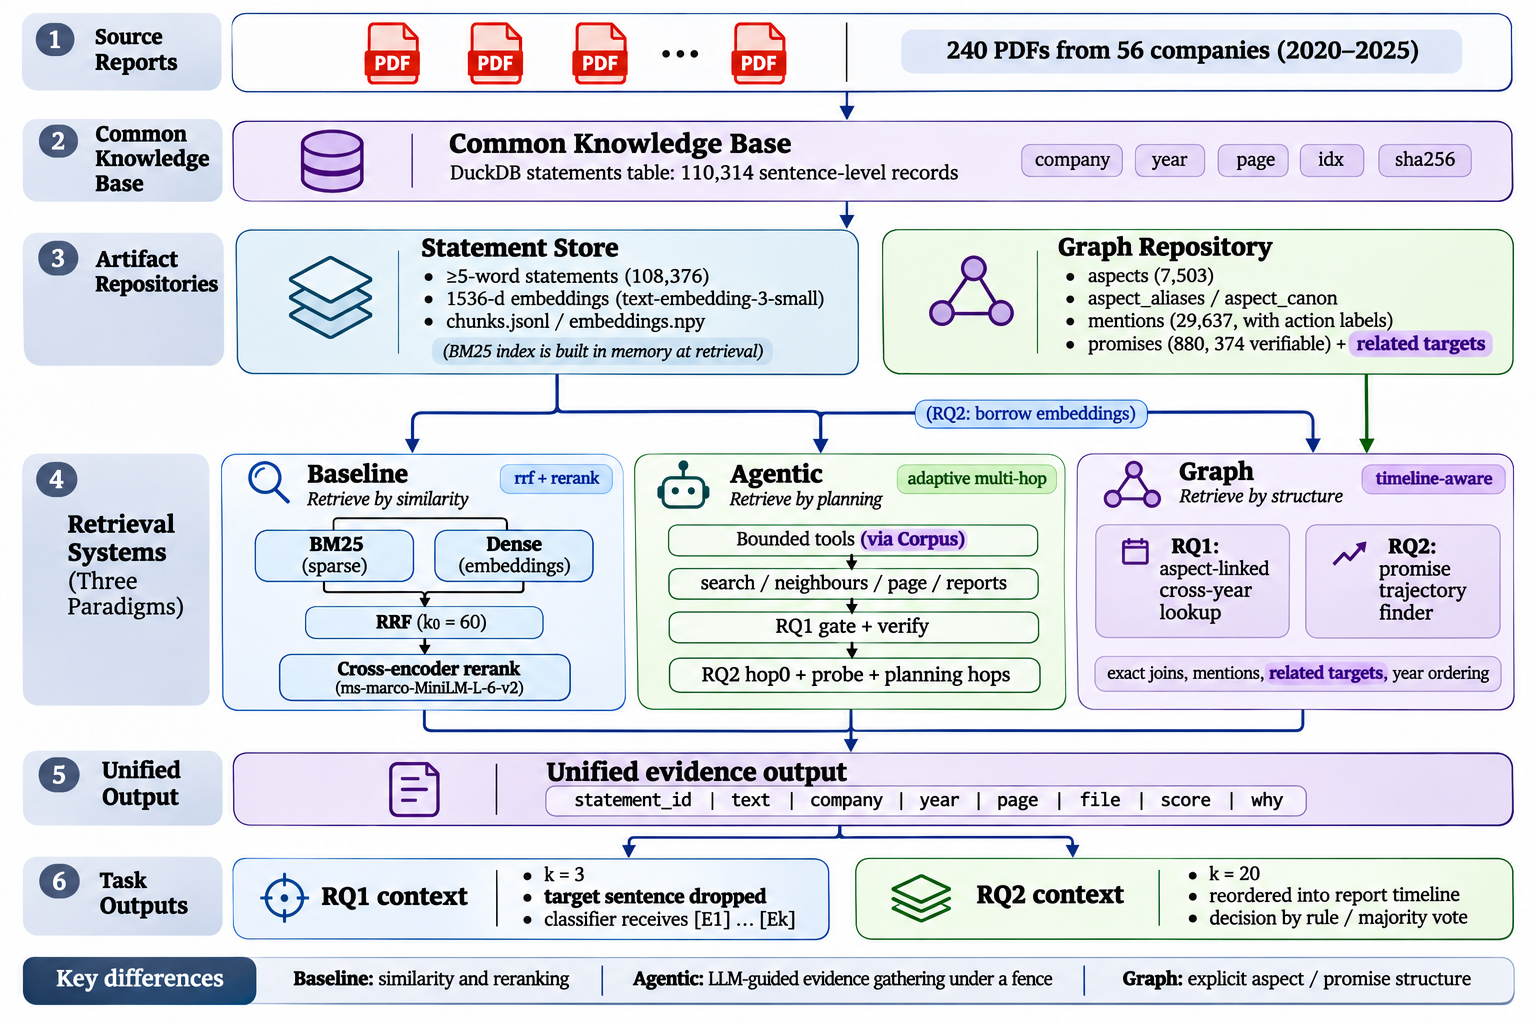
\includegraphics[width=\textwidth]{figures/flowchart.png}
\caption{From the reports to the two task contexts. One DuckDB table of 110,314 statements (sentences, table rows and metric lines alike) feeds the statement store (chunks and their vectors; the 200-word passage store of the ablation is not shown) and the temporal claim graph; the three retrievers read them and return one kind of evidence record; RQ1 hands at most three spans, the target sentence dropped, to the shared classifier, RQ2 at most twenty statements in report order to the shared judge. The agentic retriever reads the statement store only, never the graph.}
\label{fig:arch}
\end{figure*}

Figure~\ref{fig:arch} shows the pipeline: the reports are parsed once into statements, which feed the chunk stores and the claim graph; three retrievers read them and hand one shared classifier (RQ1) or one shared judge (RQ2) the same kind of evidence record.

\subsection{Retrievers}

\paragraph{Hybrid retriever.}
\label{sec:hybrid}
The baseline (Figure~\ref{fig:arch}, left) is built from parts, not a hosted service: an in-process Okapi BM25 index ($k_1 = 1.5$, $b = 0.75$) over the contextualised chunks and cosine search over the L2-normalised vectors (pgvector HNSW in the shared deployment), the top 50 of each fused by reciprocal rank fusion and the fused top 20 re-ranked by the cross-encoder on CPU. A mode switch (\texttt{bm25}, \texttt{dense}, \texttt{rrf}, \texttt{rrf+rerank}) runs the ablation through one code path; metadata filters restrict retrieval to the same report, the same company excluding the target's year, or a year window, and the target sentence is never returned.

\paragraph{Temporal claim graph.}
\label{sec:graph}
Finding the same company's statements on an aspect in other years, following a commitment forward and detecting a dropped target are joins, not similarity problems (without a company filter, templated ESG prose retrieves other companies' sentences: Q5 in Table~\ref{tab:five-queries}). Besides the aspects, mentions and promise tables of Figure~\ref{fig:arch}, the graph holds 8,524 \texttt{follows\_up} edges to later statements of the same company and aspect. LLM extraction passed its gate on the gold sentences (partial-match F1 0.649, category accuracy 0.903), but canonicalising the free-text aspects did not (best pairwise precision 0.597 against a gate of 0.80), so cross-year edges rest on morphological normalisation only. The graph arms return page-cited statements: \cond{cross\_year\_graph} joins the item's aspect to the company's other-year statements (coverage 0.40 on dev, 9\,ms), and \cond{cross\_year\_fused} fills to $k$ with BM25 over them (coverage 0.89, 20\,ms).

\paragraph{Agentic retriever.}
\label{sec:agentic}
A bounded planner calls the corpus tools of Figure~\ref{fig:arch} (filtered search, neighbours, page, reports), never the graph; code rejects any query outside the company or year window, and the agent never proposes a label or an outcome. For RQ1, a first \emph{gate} call asks whether the sentence has a gap another passage could close (an unresolved reference, an unclear actor); if not, the classifier sees exactly what \cond{sentence\_only} sees, and if so the planner writes the gap as a question with keyword queries and a \emph{verifier} keeps only the passages that answer it. For RQ2 it starts from the trajectory finder's per-year reading budget (Section~\ref{sec:rq2-evidence}; on its own the \emph{fixed-budget} arm), runs one search for a moved or dropped deadline, and takes up to two planner steps for what is still missing. An earlier version that fused the planner's queries cost 3.2$\times$ a plain search and mostly re-found the same statements.

\subsection{Classifier and promise judge}

\paragraph{Shared classifier (RQ1).}
\label{sec:classifier}
The supervised A3CG models and COGLM are the strongest published classifiers, but they read one sentence and cannot be conditioned on retrieved evidence without retraining, while RQ1 needs the \emph{same} classifier under every evidence condition. We therefore use one zero-shot LLM classifier (\chatmodel{}, low reasoning effort, temperature 0) whose prompt encodes the A3CG guideline, including the three \emph{indeterminate} sub-rules, and reads up to three evidence spans. On A3CG's released test splits with the gold aspect given it scores macro-F1 0.748 (0.714 / 0.723 averaged over the seen / unseen folds), a reference rather than a like-for-like comparison. \emph{Grounding}: it returns a label, a short rationale and page-resolved citations, at no cost in accuracy (paired $p$ 0.27--1.00 against a one-word answer). \emph{Self-consistency}: every condition runs three times uncached and the majority vote is reported.

\paragraph{Promise extraction (RQ2).}
\label{sec:promises}
An LLM extracts span, metric, quantity, unit, baseline and deadline from the 3,164 statements with a future year and a commitment cue; non-verbatim spans and past deadlines are rejected, leaving 1,273 targets (a smaller in-repo extractor agrees at \kappaval{} 0.79), merged across years into 880 promises. A promise is \emph{checkable} if it was stated before its deadline, the deadline is $\le 2025$ with a report for that year or the next, and its metric is concrete: 374 promises from 32 companies (Figure~\ref{fig:funnel}).

\begin{figure}[t]
\centering
\begin{tikzpicture}[font=\scriptsize, node distance=2mm,
  st/.style={draw, rounded corners=2pt, fill=blue!6, align=center, inner sep=3pt, text width=6.4cm}]
  \node[st] (a) {110,314 parsed statements};
  \node[st, below=of a] (b) {3,164 candidates: a future year and a commitment cue};
  \node[st, below=of b] (c) {1,273 validated dated targets (sub-agents; the small model finds 1,462, $\kappa$ 0.79)};
  \node[st, below=of c] (d) {880 promises: restatements merged, \texttt{related} targets linked};
  \node[st, below=of d] (e) {374 checkable: deadline $\le$ 2025, stated before it, a report for it};
  \node[st, fill=green!8, below=of e] (f) {373 gold outcomes, dev 123 / test 250: 137 by the human pair ($\kappa$ 0.84), 236 by the model pair, adjudicated};
  \foreach \x/\y in {a/b,b/c,c/d,d/e,e/f} \draw[-{Latex[length=1.6mm]}] (\x) -- (\y);
\end{tikzpicture}
\caption{The promise pipeline from statements to the gold set.}
\label{fig:funnel}
\end{figure}


\paragraph{Evidence.}
\label{sec:rq2-evidence}
The \emph{trajectory finder} ranks every statement of every later report with BM25 and dense retrieval, takes a budget per report year (6 statements from the first report at or after the deadline, 3 from the next, 2 from each earlier one), adds the neighbours of the two best hits in the deadline report (a flattened target table puts the result beside the target) and up to three related targets, and shows everything in report order: 11.6 statements per promise. The hybrid baseline returns its top 20 in the same window.

\paragraph{Judge.}
The judge asks of each statement whether it is about this target, only its metric, or neither; whether it reports the deadline year's result as met or missed; and whether it moves the target to a later date or drops it. Beyond literal restatements, three readings count a statement as being about the target: the company's own account of the same matter in other words (\texttt{proxy}), a stated part delivery (\texttt{partial}, counted as a miss) and the deadline year's figure compared with the target in code (\texttt{figure}). A fixed rule then decides: a \emph{met} and no \emph{missed} on this target $\to$ achieved; otherwise a later or no date on a non-annual target $\to$ failed (revised); otherwise a \emph{missed} $\to$ failed; otherwise any statement on the target or its metric from the deadline year on $\to$ unclear; otherwise disappeared. The outcome is the majority of three runs (no majority: unclear). The questions, the rule and the three readings were settled on the development split's errors, so development numbers are optimistic and the test split is the measure.

\subsection{User interface and five timed queries}
\label{sec:serving}

A FastAPI service (\texttt{gw-serve}) exposes classification, retrieval, trajectory and graph endpoints with one router per system, and every response that shows text carries its company, year and page. The Streamlit front end (Figure~\ref{fig:ui}) lets the user choose the question, the system, the evidence condition, $k$ and the number of votes, run a development item or a query of their own step by step with a live timer, and see the answer against the gold with its rationale and citations, every evidence span with its source, the retrieval, generation and end-to-end time, tokens and cost, and any cited page rendered from the raw report; for RQ2 the evidence is a timeline by report year with the judge's label on each statement. Caching is off, so a timing is a real timing.

\begin{figure*}[t]
\centering
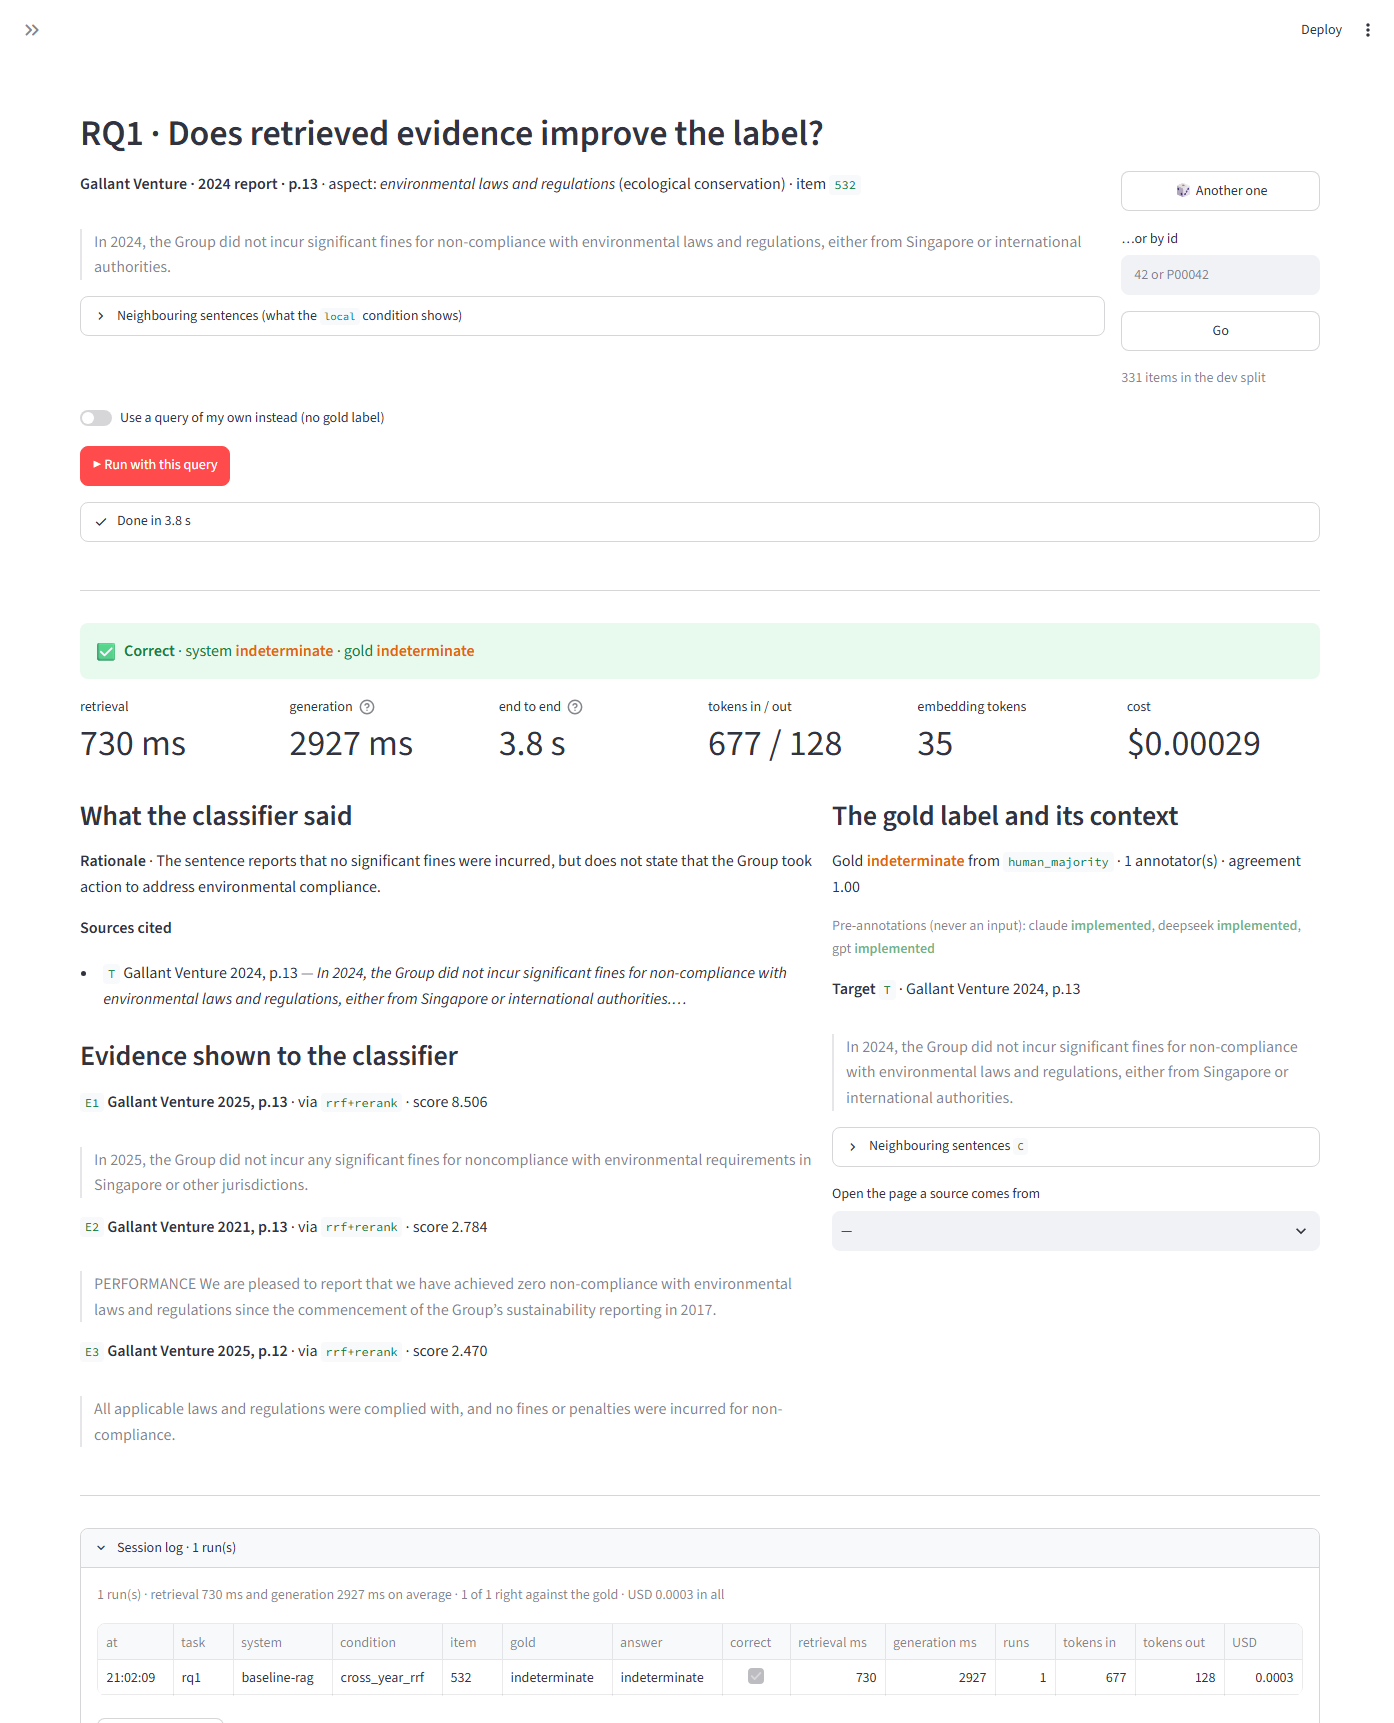
\includegraphics[width=0.495\textwidth]{figures/ui-rq1.png}\hfill
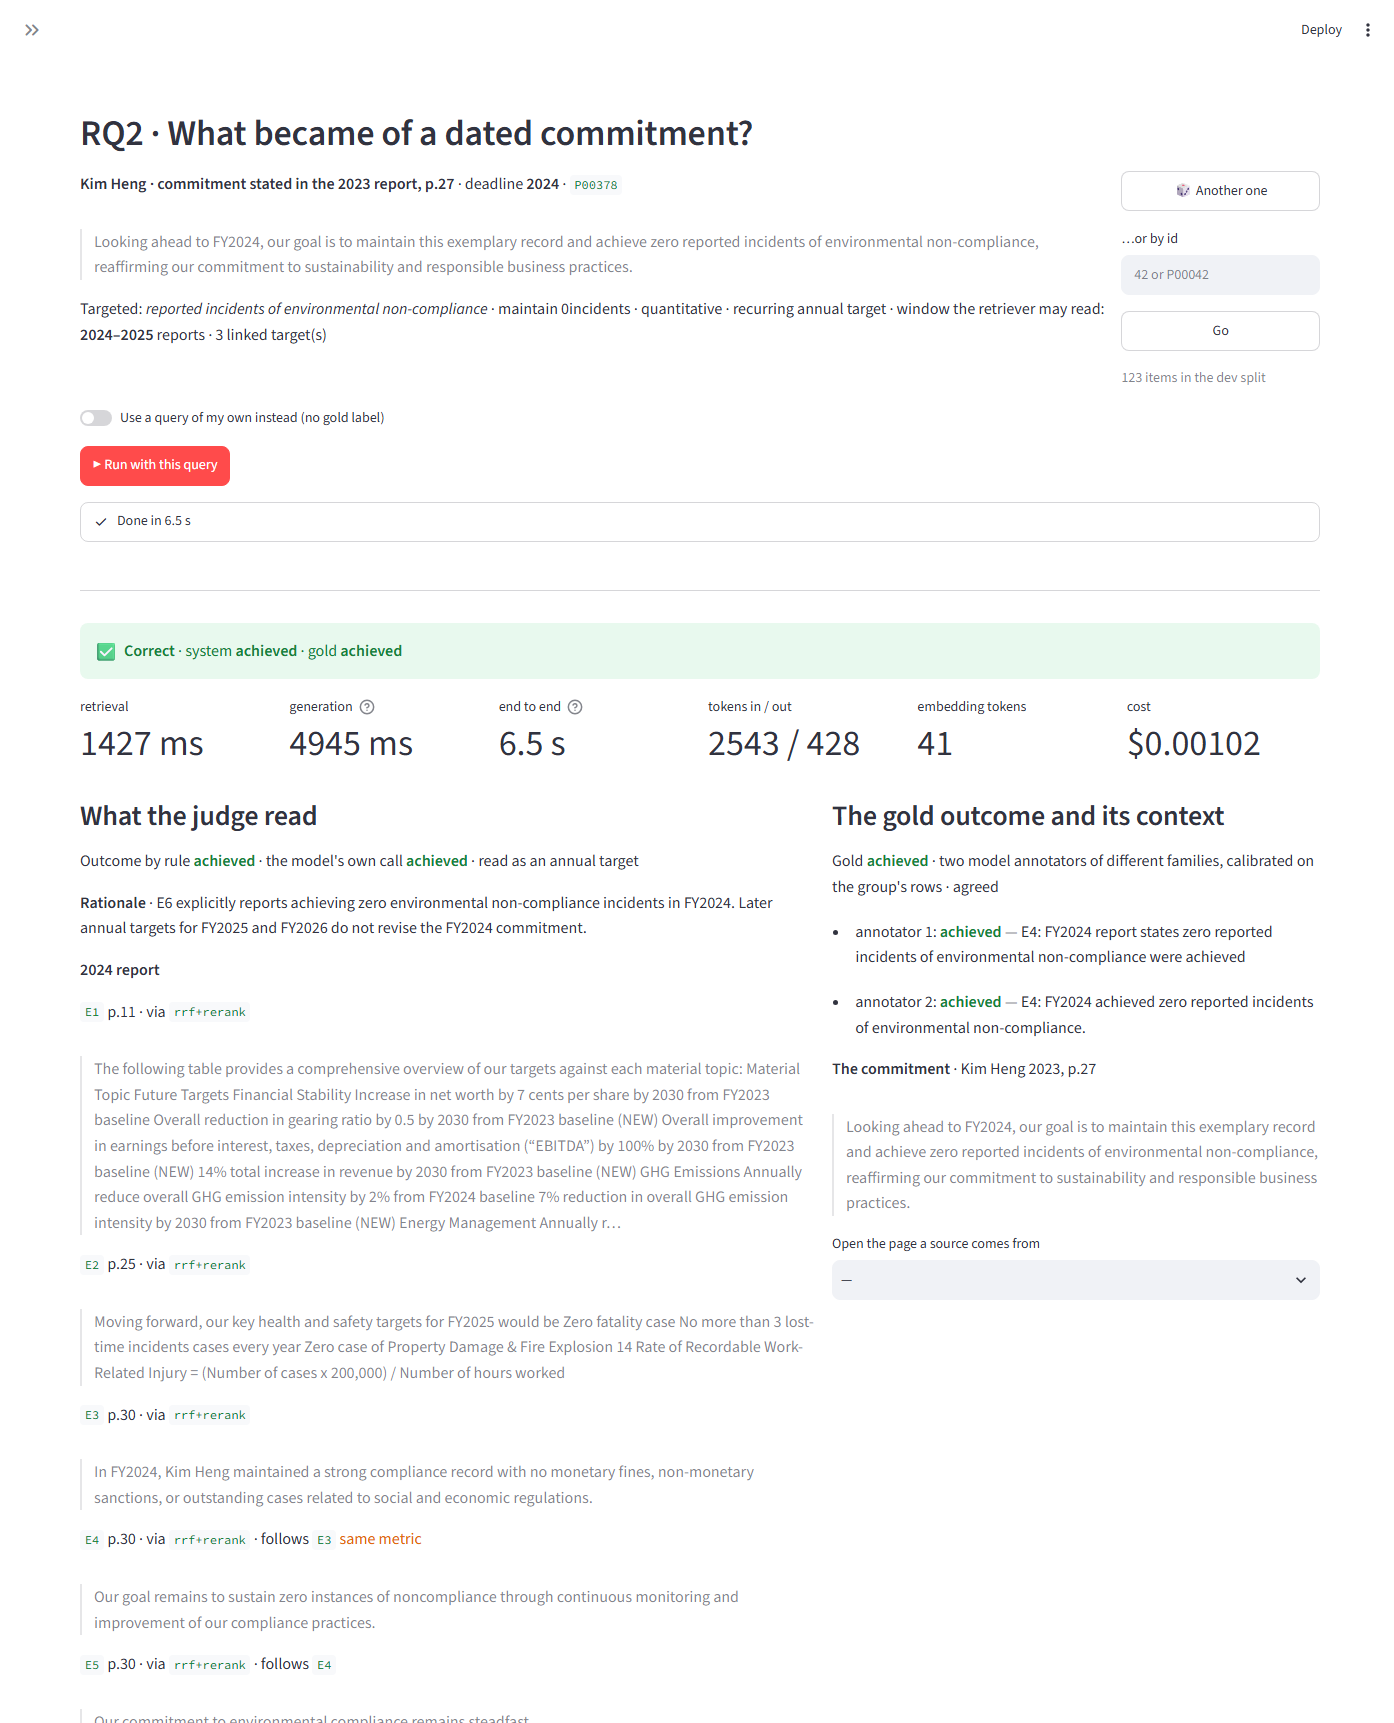
\includegraphics[width=0.495\textwidth]{figures/ui-rq2.png}
\caption{The demo front end (\texttt{frontend/}, Streamlit). Left: an RQ1 development item run through the hybrid baseline under \cond{cross\_year\_rrf}; the label against the gold, the timings, tokens and cost, the rationale with its citations, and the three evidence spans with their source. Right: an RQ2 promise run under \cond{promise\_window}; the outcome against the gold and the evidence as a timeline by report year with the judge's label on each statement.}
\label{fig:ui}
\end{figure*}

Table~\ref{tab:five-queries} runs five queries that stand for the user task in every retrieval mode. BM25 answers in 2--4\,ms inside a company filter and 20\,ms over the whole store; dense and hybrid add about 20\,ms when the query vector is cached (an uncached query adds the embedding round trip, 190--730\,ms p50); the CPU cross-encoder adds 100--550\,ms. The re-ranked lists are the most readable: Q3 returns each year's annual target sentence in order, Q2 the 89\% certification figure beside the 2021 target sentence, and Q5 shows why the company filter exists: without it, the nearest neighbours of a net-zero commitment are other issuers' near-identical sentences, and the top hit is a national target quoted in an issuer's report: provenance is not attribution, the actor question that the RQ1 classifier and the promise extractor both face.

\begin{table*}[t]
\centering\small
\begin{tabular}{@{}lL{3.4cm}rrrrL{6.2cm}@{}}
\toprule
& query (filter) & BM25 & dense & hybrid & +rerank & top hit after re-ranking \\
& & ms & ms & ms & ms & \\
\midrule
Q1 & Scope 3 greenhouse gas emissions reporting (Gallant Venture, 2022--2025) & 3.8 & 19.2 & 23.3 & 571.6 & 2023 p.26 ``Disclose Scope 1, 2, and, if appropriate, Scope 3 greenhouse gas (GHG) emissions and the related risks.'' \\
Q2 & 100\% ISPO certification of mills and estates (Indofood Agri, 2021--2025) & 2.3 & 20.5 & 23.5 & 430.0 & 2024 p.43 ``Sustainability certification of all estates' hectarage is ISPO certified \ldots 89\%''; second hit 2021 p.11 ``we aim to have 100\% of our mills and estates ISPO certified by 2023.'' \\
Q3 & electricity consumption per square foot target (Old Chang Kee, 2021--2025) & 2.9 & 19.3 & 22.3 & 130.1 & 2021 p.14 ``Our target is to maintain or lower our electricity consumption (kwh) per square foot in FY2022.''; the FY2023 and FY2024 target sentences follow \\
Q4 & solar rooftops installed at distribution centers (ThaiBev, 2023--2025) & 2.4 & 20.5 & 21.0 & 180.9 & 2023 p.169 ``In 2023, ThaiBev installed solar rooftops at two distribution centers in Nakhon Ratchasima and Surat Thani.'' \\
Q5 & commitment to achieve net zero emissions by 2050 (no filter) & 20.2 & 22.4 & 44.6 & 125.4 & ThaiBev 2025 p.31 ``Thailand has committed to achieving Net-Zero greenhouse gas emissions by 2050.''; then CSE Global 2025, Centurion 2025 \\
\bottomrule
\end{tabular}
\caption{Five example queries (Question 2): median of three calls after a warm-up, $k = 5$, statement store \texttt{d8a62bfe40c6}, one machine, CPU re-ranker. End-to-end classification of an item, retrieval plus one classifier call, runs at 2.8--3.8\,s p50 in the evaluation runs (Table~\ref{tab:rq1-cost}).}
\label{tab:five-queries}
\end{table*}

\subsection{Retrieval innovations and the queries they fixed}
\label{sec:innovations}
Five changes beyond the course pipeline each fixed a specific failure. (1)~\emph{Contextual headers}: prefixing each chunk with company, year and page gives BM25 and the encoder the company name a bare table row lacks. (2)~\emph{Company, year and cross-year filters}: every RQ1 retrieval arm is scoped to the company and the cross-year arms exclude the target's report year, every RQ2 arm reads only the window after the promise (Q5). (3)~\emph{The statement as the unit}: passages are never better evidence than statements and cost more to retrieve and read (Section~\ref{sec:rq1-ablation}). (4)~\emph{Every statement in the dense index}: the first promise evidence fused a complete BM25 ranking with a dense ranking over the 71,342 sentence-shaped statements only; under RRF a statement first in one list ($1/61$) ranks below one thirtieth in both ($2/90$), so result lines ranked first to third by BM25 were cut (e.g.\ ThaiBev's ``installed solar rooftops at two distribution centers'' fell from first to seventh; Table~\ref{tab:fixed-queries}). With both rankings complete, a budget per report year and neighbours, six of the eight hand-found answers are shown and the human-verified \emph{unclear} share fell from 49\% to 31\%. (5)~\emph{The graph join and the trajectory finder}: an exact join on (company, aspect, year) answers in 9--20\,ms what the hybrid path answers in 190--730\,ms, and ordered, budgeted reading of later reports lets the judge read 11.7 statements instead of 20 at the same accuracy (Section~\ref{sec:rq2-gold}).


\subsection{Rank-aware retrieval evaluation}
\label{sec:rq1-retrieval}
Table~\ref{tab:retrieval} scores the retrievers on 80 development queries, 78 of which score: 30 sentences asked over the company's other years (two came from issuers with a single report in the store, so no cross-year configuration could return anything), 30 company-and-aspect lookups and 20 topic queries over all companies. Six configurations contributed their top 10 to one pool of 1,658 (query, statement) pairs, graded once on a 0--3 scale by the group's model under a fixed prompt (relevant: grade $\ge 2$), so the numbers compare configurations under one judge rather than measure absolute quality. The re-ranked hybrid is the best or tied-best configuration; BM25 alone trails it by 0.09--0.11 nDCG@10 with the paired interval clear of zero; dense retrieval and plain fusion are within its interval, and the re-ranker's gain shows mostly in MRR (0.913 to 0.934 overall, 0.809 to 0.896 on the sentence queries). Wrong-company@10 is zero for every configuration. The graph arm is sparse rather than wrong: it returns 1.7 statements of 10, and the first is usually relevant (MRR 0.90 on aspect queries); filled with BM25 it is within the re-ranked hybrid's interval on company queries, with no embedding call.

\begin{table*}[t]
\centering\scriptsize
\setlength{\tabcolsep}{3.5pt}
\begin{tabular}{@{}lrrrrrrrrl@{}}
\toprule
 & & \multicolumn{4}{c}{all 78 queries} & \multicolumn{3}{c}{nDCG@10 by query type} & \multicolumn{1}{c}{$\Delta$nDCG@10 vs.\ re-ranked} \\
\cmidrule(lr){3-6}\cmidrule(lr){7-9}\cmidrule(l){10-10}
configuration & returned & P@5 & R@10 & MRR & nDCG@10 & sentence (28) & aspect (30) & topic (20) & \multicolumn{1}{c}{company queries (58)} \\
\midrule
BM25 & 10.0 & 0.728 & 0.471 & 0.886 & 0.706 & 0.570 & 0.749 & 0.832 & $-0.106$ [$-0.150$, $-0.061$] \\
dense & 10.0 & 0.805 & 0.564 & 0.900 & 0.793 & 0.699 & 0.809 & 0.902 & $-0.013$ [$-0.056$, $+0.032$] \\
RRF (BM25 + dense) & 10.0 & 0.785 & 0.543 & 0.913 & 0.782 & 0.677 & 0.826 & 0.862 & $-0.014$ [$-0.048$, $+0.018$] \\
RRF + re-ranker & 10.0 & 0.797 & 0.555 & 0.934 & 0.800 & 0.705 & 0.827 & 0.891 & reference \\
graph (G) & 1.7 & 0.228 & 0.108 & 0.490 & 0.209 & 0.182 & 0.374 & -- & $-0.487$ [$-0.561$, $-0.414$] \\
graph + BM25 fused (G) & 7.4 & 0.567 & 0.409 & 0.664 & 0.547 & 0.653 & 0.812 & -- & $-0.033$ [$-0.094$, $+0.026$] \\
\bottomrule
\end{tabular}
\caption{Rank-aware retrieval metrics on pooled, model-made relevance grades (run \run{retrieval/dev-pooled-model-judged}; 80 development queries, of which 78 had candidates and score, $k = 10$, relevant = grade $\ge 2$, recall against the pool). The two graph arms need a company and return nothing on the topic queries, so their overall columns count those as zero; the last column is the paired bootstrap mean and 95\% interval of the difference in nDCG@10 against the re-ranked hybrid over the 58 company queries. Wrong-company@10 is 0 for every configuration.}
\label{tab:retrieval}
\end{table*}

% =============================================================================================
\section{Evaluation Protocol}
\label{sec:metrics}

\paragraph{Evidence conditions.}
\label{sec:conditions}
Every RQ1 arm uses one classifier, prompt and budget ($k = 3$ spans of at most 800 characters) and differs only in the evidence: none (\cond{sentence\_only}), the neighbouring sentences, hybrid retrieval from the same report or other years, the graph join with or without BM25 fill, or the agent (Table~\ref{tab:conditions}, Appendix). Any returned span that \emph{is} the target sentence is dropped. Every RQ2 arm returns at most $k = 20$ statements from the window $y_0{+}1$ to $d{+}1$ to the shared judge.

\paragraph{Metrics.}
RQ1: macro-F1 over the three action labels on rows whose gold label is an action (274 dev, 556 test), per-label precision, recall and F1, and F1 for detecting \emph{none}, because evidence can talk a model into inventing an aspect. RQ2: accuracy, \kappaval{} and macro-F1 over the four outcomes, plus \emph{over-commitment} (a verdict where the gold is unclear), \emph{under-commitment} (unclear where the gold has a verdict) and the precision of the verdicts given. RAG: RAGAS faithfulness, answer relevance, context precision and context relevance, implemented in-house and calibrated against a human. Performance: latency, items per second, tokens and USD per 1,000 items (0.20 / 1.20 USD per million input / output tokens).

\paragraph{Comparison and protocol.}
An identical configuration does not reproduce its score (three sentence-only votes on dev: 0.7397 / 0.7498 / 0.7580), so arms are compared only by the paired McNemar test on majority votes over the same items, reported as flips wrong$\to$right / right$\to$wrong. Dev is for tuning; each test split was read once with the comparisons frozen beforehand (RQ1 on 2026-11-05; RQ2 on 2026-10-31 and 2026-11-04). Every number names its published run and snapshot hash. Chat model \chatmodel{} at low reasoning effort and temperature 0; embeddings \embmodel{}; re-ranker \reranker{} on CPU.

\subsection{Data and code}
\label{sec:resources}
Appendix~\ref{app:resources} links the code repository, whose README explains how to install and run everything, the archive with the knowledge base, the evaluation sets, the published runs, predictions and judge outputs, and the annotation sheet. The \texttt{uv} workspace has one package per system, the Streamlit demo in \texttt{frontend/} and 139 offline unit tests.

% =============================================================================================
\section{Results for RQ1}
\label{sec:rq1}

\subsection{Does evidence change the label?}
\label{sec:rq1-main}
\label{sec:rq1-test}
Table~\ref{tab:rq1-summary} gives the main arms on both splits. On dev, where three sentence-only runs differ by up to 0.018, the best evidence arm, hybrid retrieval from the company's other years, adds 0.037 to its own sentence-only vote ($p = 0.21$), and the graph is not distinguishable from plain hybrid retrieval ($+6 / {-11}$, $p = 0.33$). The test split confirms this: \textbf{no evidence condition of any system raises macro-F1 by more than 0.015 over its own sentence-only vote, and every significant paired difference is a loss}. The losses come from \emph{none} detection: shown neighbouring sentences or retrieved statements, the model more often reads an aspect--action pair into a sentence the annotators said has none (\emph{none} F1 falls from 0.83--0.84 to 0.66--0.80, significantly for six of the fourteen evidence arms, e.g.\ $+20 / {-36}$ for cross-year hybrid evidence, $p = 0.044$). The graph arm, which shows evidence on only 42\% of items, keeps \emph{none} F1 at 0.83 and is ahead of cross-year hybrid evidence ($+32 / {-15}$, $p = 0.019$), largely because it shows evidence less often. Per label (Table~\ref{tab:rq1-labels}), cross-year evidence lifts \emph{indeterminate} recall from 0.50 to 0.57 on dev, but in every arm a quarter of the \emph{indeterminate} items are read as \emph{implemented}.

\begin{table*}[t]
\centering\scriptsize
\setlength{\tabcolsep}{4.5pt}
\begin{tabular}{@{}lrrrrrrrr@{}}
\toprule
 & \multicolumn{2}{c}{dev (331 items)} & \multicolumn{6}{c}{test (669 items)} \\
\cmidrule(lr){2-3}\cmidrule(l){4-9}
arm (run) & vote & $p$ & vote & none F1 & flips vs own S-only & $p$ & retr.\ p50 & USD/1k \\
\midrule
sentence only (B) & 0.7397 & -- & 0.7644 & 0.833 & -- & -- & -- & 0.211 \\
neighbouring sentences (B) & 0.7617 & 0.82 & 0.7701 & 0.693 & $+23 / {-40}$ & 0.043 & -- & 0.247 \\
hybrid, same report (B) & 0.7442 & 0.68 & 0.7731 & 0.723 & $+21 / {-33}$ & 0.134 & 500 ms & 0.257 \\
hybrid, other years (B) & 0.7767 & 0.21 & 0.7662 & 0.730 & $+20 / {-36}$ & 0.044 & 173 ms & 0.253 \\
graph, other years (G) & 0.7449 & 0.77 & 0.7708 & 0.831 & $+12 / {-11}$ & 1.00 & 6 ms & 0.225 \\
graph + BM25 fused (G) & 0.7668 & 1.00 & 0.7582 & 0.774 & $+16 / {-29}$ & 0.072 & 9 ms & 0.248 \\
agent, other years (A) & 0.7609 & 0.82 & 0.7644 & 0.796 & $+15 / {-26}$ & 0.117 & 2.9 s & 0.468 \\
agent, every report (A) & 0.7645 & 0.65 & 0.7734 & 0.761 & $+19 / {-30}$ & 0.152 & 2.3 s & 0.484 \\
\bottomrule
\end{tabular}
\caption{Main RQ1 arms: action macro-F1 of the majority vote over three uncached repeats, cited classifier, statement store. $p$ and flips are the paired McNemar test against the same run's sentence-only vote (dev: B 0.7397, G 0.7498, A 0.7686; test: B 0.7644, G 0.7663, A 0.7706). Runs: (B) \run{baseline/statement-hybrid-cited}, (G) \run{graph/graph-arms-cited}, (A) \run{agentic/rq1-dev-all-arms} and their test runs; latency and cost on test (the agentic run used 8 retrieval workers, so its latency includes queueing). Full tables with intervals and the passage-store runs: Tables~\ref{tab:rq1-main}, \ref{tab:rq1-agentic} and~\ref{tab:rq1-test}.}
\label{tab:rq1-summary}
\end{table*}

\begin{table}[t]
\centering\footnotesize
\setlength{\tabcolsep}{4pt}
\begin{tabular}{@{}llrrr@{}}
\toprule
arm & label & P & R & F1 \\
\midrule
\multirow{3}{*}{sentence only} & implemented & 0.796 & 0.860 & 0.827 \\
 & planning & 0.740 & 0.864 & 0.797 \\
 & indeterminate & 0.735 & 0.500 & 0.595 \\
\midrule
\multirow{3}{*}{hybrid, other yrs} & implemented & 0.805 & 0.882 & 0.842 \\
 & planning & 0.803 & 0.864 & 0.832 \\
 & indeterminate & 0.774 & 0.569 & 0.656 \\
\bottomrule
\end{tabular}
\caption{Per-label precision, recall and F1 of the majority vote (dev; supports 136 / 66 / 72). In every arm, including graph + BM25 (not shown), a quarter of the \emph{indeterminate} items are read as \emph{implemented} (23--25 of 72), the LLM failure mode A3CG reports.}
\label{tab:rq1-labels}
\end{table}

\subsection{Why so little: the classifier rarely uses what it is given}
\label{sec:rq1-why}
The classifier cites a retrieved span in only 1--9\% of items, and the RAG-metric judge (Table~\ref{tab:ragas}) finds the rationales faithful (0.96--0.98 of their atomic statements supported by the sources shown) and a minority of the retrieved statements relevant (context relevance 0.27--0.40). A human calibration of the judge on 186 blind rows found it strict on faithfulness (agreement 0.976) and lenient on relevance by about 1.7$\times$ (agreement 0.831), so the corrected context relevance is about 0.16--0.24. For labelling what a sentence says, the sentence carries the answer.

\begin{table}[t]
\centering\scriptsize
\setlength{\tabcolsep}{3pt}
\begin{tabular}{@{}lrrrr@{}}
\toprule
condition & faith. & ans.\ rel. & ctx.\ P & ctx.\ rel. \\
\midrule
sentence only & 0.964 & 0.574 & -- & -- \\
hybrid, same report & 0.976 & 0.563 & 0.497 & 0.369 \\
hybrid, other years & 0.973 & 0.568 & 0.371 & 0.286 \\
\midrule
sentence only, test & 0.970 & 0.570 & -- & -- \\
hybrid, same report, test & 0.980 & 0.567 & 0.527 & 0.402 \\
hybrid, other years, test & 0.975 & 0.569 & 0.335 & 0.273 \\
\midrule
judge--human agreement & 0.976 & -- & -- & 0.831 \\
\bottomrule
\end{tabular}
\caption{Answer-level RAG metrics, LLM-judged on repeat 0: dev (run \run{baseline/statement-hybrid-cited}, 331 items) and test (\run{baseline/statement-hybrid-cited-test}, 669 items), and the human calibration of the judge (186 dev rows; the judge is lenient on context relevance by 1.7$\times$). Answer relevance is comparable across conditions, not against 1.0.}
\label{tab:ragas}
\end{table}

\subsection{Ablations of the downstream innovations}
\label{sec:rq1-ablation}

\paragraph{Statements versus passages.}
\label{sec:rq1-unit}
Table~\ref{tab:rq1-unit} pairs the 200-word passage store against the statement store on the same items. Each split favours statements once and ties once (dev, other years: $p = 0.043$; test, same report: $p = 0.017$); neither ever favours passages, and statements are also cheaper (USD 0.25 against 0.28--0.29 per 1,000 items) and faster to retrieve (173--500\,ms against 830--1,120\,ms on test).

\begin{table}[t]
\centering\scriptsize
\setlength{\tabcolsep}{3pt}
\begin{tabular*}{\columnwidth}{@{}l@{\extracolsep{\fill}}rrrrrr@{}}
\toprule
 & \multicolumn{3}{c}{dev (331 items)} & \multicolumn{3}{c}{test (669 items)} \\
\cmidrule(lr){2-4}\cmidrule(lr){5-7}
evidence from & pass. & stmt. & $p$ & pass. & stmt. & $p$ \\
\midrule
same report & 0.750 & 0.744 & 1.00 & 0.739 & \textbf{0.773} & \textbf{0.017} \\
other years & 0.740 & \textbf{0.777} & \textbf{0.043} & 0.774 & 0.766 & 1.00 \\
\bottomrule
\end{tabular*}
\caption{Granularity ablation: vote macro-F1 with three passages (pass.) or three statements (stmt.) of hybrid evidence, paired on the same items (McNemar $p$). Runs \run{baseline/passage-hybrid-cited}, \run{baseline/statement-hybrid-cited} and their test runs.}
\label{tab:rq1-unit}
\end{table}

\paragraph{Agentic retrieval.}
\label{sec:rq1-agentic}
The gate opens on 69 of 331 dev and 155 of 669 test sentences; on the rest the agentic and sentence-only arms read one identical prompt, and their dev votes still flip $+4 / {-6}$, the model's own noise. The spans the agent hands over are cited on 12--24\% of the items given evidence, against 0.5--8\% for plain retrieval, but the label does not move (test, \cond{company\_agentic} against sentence-only: $+19 / {-30}$, $p = 0.15$), and the gate's call on every item doubles the cost (USD 0.47--0.48 against 0.21--0.26 per 1,000 items). Four ablations of the agent (no verifier, three hops, cross-encoder selection, neighbours kept) stay inside the noise. A dev finding that neighbouring sentences help context-dependent sentences ($+9 / {-0}$ on 75 items, one of ten slice comparisons) did not replicate on test ($+8 / {-8}$).

\subsection{Speed, cost and scalability}
\label{sec:rq1-cost}
A classifier call takes 2.7--3.1\,s p50 regardless of evidence; retrieval adds 9--20\,ms through the graph and 190--730\,ms through the hybrid path (a query embedding round trip and a CPU cross-encoder pass), so an item takes 2.8--3.8\,s end to end, and throughput at the classifier's concurrency of eight is 2.3--2.7 items per second (Table~\ref{tab:rq1-cost}). Cost is USD 0.21--0.30 per 1,000 items (540--990 input and 86--105 output tokens); judging all 374 promises three times costs USD 1.5--1.9. The 108,376 vectors take 660\,MB in memory; the Postgres backend serves them through an HNSW index for a shared deployment, and the per-company filters keep the dense candidate set small.

% =============================================================================================
\section{Results for RQ2}
\label{sec:rq2}

\subsection{The judge on the human checks}
\label{sec:rq2-judge}
Two human check sheets, weighted to their pools, score the first system and the decomposed judge (Table~\ref{tab:rq2-checks}). Accuracy on the reported classes is 0.82 in both; what changed is \emph{where} the system is wrong. The first judge, naming the outcome directly, gave a verdict on 31\% of the commitments the annotator could not settle. With per-statement questions and the rule, on 60 held-out rows, that over-commitment fell to 14\% and the verdicts given are right 85\% of the time, at the price of 15\% of settled commitments left \emph{unclear}. Ablating the rule on the 74 rows the prompt was tuned on, the model's own outcome in the same reply reaches 0.81 and the rule 0.88--0.92, so the rule adds to the per-statement questions. The three readings added afterwards (\texttt{proxy}, \texttt{partial}, \texttt{figure}) were checked by the group against the same sheets and found no less reliable. The judge is noisy (16\% of promises change outcome across three runs), hence the majority vote.

\subsection{Retrieval arms against the gold set}
\label{sec:rq2-gold}
\label{sec:rq2-test}
Table~\ref{tab:rq2-summary} compares the four retrievers under the shared judge, above two floors: answering the development split's majority class (\emph{achieved}) for every promise, and the model shown the commitment alone, with no retrieved statement (majority of three replies). The majority floor scores 0.496 on dev and 0.580 on test and gives a verdict on every promise a reader cannot settle; the model without evidence abstains on 97\% of promises (0.195 and 0.284), giving nine verdicts on test, eight of them right. Every retrieval arm is above both on every promise set (the finder against the majority floor on test $+75 / {-19}$, against the model without evidence $+147 / {-17}$, both $p < 0.001$): the question is not answerable from the commitment alone. On dev the trajectory finder and the agent tie at 0.837, the hybrid top 20 is at 0.813 and the fixed budget at 0.870, all within the noise of a judge settled on this split's errors (eight repeats on the fixed budget's evidence range 0.829--0.870); the finder reads 11.6 statements where the hybrid reads 20, so its judgements are cheaper and steadier. Because the same hybrid configuration scored 0.816 and 0.748 in two test batches on different machines, test arms are compared only within the second batch, where all four ran on one machine. There the finder (0.804) and the agent (0.800) lead the fixed budget (0.768) and the hybrid baseline (0.748): the finder is ahead of the baseline ($+24 / {-10}$, $p = 0.024$, uncorrected, the one retrieval comparison on test below 0.05) and ties the agent ($+14 / {-15}$, $p = 1.00$), which needs a planner and fifty times the retrieval latency; its verdicts are also the most often right (0.88 against 0.83--0.86). \textbf{The graph's ordered, shorter evidence is what the judge rewards}: 20 loosely ranked statements give it more to over-commit on (a verdict on 27 of the 64 gold-unclear promises against 18 for the finder).

\textbf{Retrieval is not what limits RQ2}: in 14 of the 17 checkable hybrid errors on dev the deciding phrase was already in the evidence, doubling the evidence to 40 statements lowered accuracy, and the planner's own hops added statements the judge almost never used. The lever is how the judge reads the evidence: its stricter predecessor, which counted only literal restatements of the target as being about it, scores 5 to 17 of 250 test promises lower on every arm ($p = 0.006$ on the finder's evidence, $0.020$ on the agent's; run records), by leaving settled promises unclear. That gain sits mostly on the model-annotated rows (the 115 human-labelled test rows move by at most six, the 135 model-labelled rows by 8 to 14), so part of it may be agreement between the judge's reading and the model annotators' rather than correctness, and dev overstated it (fixed budget 0.870 on dev, 0.768--0.808 on test). The agent-plus-filter pipeline chosen on dev (0.808 in the first batch) ties the fixed budget and trails the plain agent there ($+5 / {-13}$, $p = 0.096$) at twice the judging cost.

\begin{table}[t]
\centering\scriptsize
\setlength{\tabcolsep}{2pt}
\begin{tabular*}{\columnwidth}{@{}l@{\extracolsep{\fill}}rrrrrrr@{}}
\toprule
 & & \multicolumn{2}{c}{accuracy} & \multicolumn{3}{c}{test} & \\
\cmidrule(lr){3-4}\cmidrule(lr){5-7}
arm & stmts & dev & test & over & under & prec. & USD/1k \\
\midrule
majority class & -- & 0.496 & 0.580 & 64/64 & 0/186 & 0.58 & 0 \\
model, no evidence & 0 & 0.195 & 0.284 & 1/64 & 178/186 & 0.89 & 0.90 \\
\midrule
hybrid top-20 & 20.0 & 0.813 & 0.748 & 27/64 & 33/186 & 0.83 & 5.64 \\
trajectory finder (graph) & 11.6 & 0.837 & \textbf{0.804} & 18/64 & 27/186 & \textbf{0.88} & 4.56 \\
fixed budget & 11.5 & \textbf{0.870} & 0.768 & 22/64 & 29/186 & 0.84 & 4.59 \\
agent, two hops & 16.5 & 0.837 & 0.800 & 21/64 & 24/186 & 0.86 & 6.32 \\
\bottomrule
\end{tabular*}
\caption{RQ2 outcome accuracy (majority of three judge runs) on dev (123 promises) and on the second test batch (250 promises, all four arms on one machine), above the two floors (runs \run{baseline/rq2-majority-*}, \run{baseline/rq2-direct-*}). Over: verdicts given on the 64 gold-unclear test promises; under: the 186 settled test promises left unclear; prec.: share of test verdicts that are right; cost per 1,000 promises on test. The judge was settled on the dev errors, so its dev numbers are optimistic. Full tables: \ref{tab:rq2-main}, \ref{tab:rq2-test} and~\ref{tab:rq2-test-pairs}.}
\label{tab:rq2-summary}
\end{table}

\subsection{What the commitments did}
\label{sec:rq2-outcomes}
\label{sec:rq2-cases}
Figure~\ref{fig:outcomes} gives the outcome shares three ways: about half met, one in eight to nearly one in five (13--18\%) missed or re-dated, a quarter to a third unclear. The \emph{unclear} share fell from 49\% on the first evidence to 31\% on the complete evidence; the two human checks are different samples weighted to different pools, so the drop is descriptive rather than a controlled estimate, but the case studies point the same way: of the eleven commitments the first check called \emph{disappeared}, five were in the reports after all, and of ten case studies followed through every statement (Table~\ref{tab:cases}), reading the whole timeline changed the label of five. In one, Gallant Venture promised in 2022 to report Scope 3 categories ``by FY2023'' (p.34), then was ``looking into'' them (2023) and ``exploring'' them (2024, 2025): each later sentence alone is unremarkable, and only the sequence (query Q1) shows a dated commitment whose date was never replaced.


\begin{figure}[t]
\centering
\begin{tikzpicture}
\begin{axis}[
  width=\columnwidth, height=4.6cm, ybar, bar width=7pt,
  ymin=0, ymax=102, ytick={0,20,40,60}, nodes near coords, every node near coord/.append style={font=\tiny, black, /pgf/number format/fixed, /pgf/number format/precision=0}, ylabel={share of commitments (\%)}, ylabel near ticks,
  symbolic x coords={achieved,failed,unclear,disappeared}, xtick=data,
  x tick label style={font=\scriptsize}, y tick label style={font=\scriptsize}, ylabel style={font=\scriptsize},
  legend style={font=\tiny, at={(0.99,0.99)}, anchor=north east, draw=none, fill=white, legend columns=1, cells={anchor=west}},
  enlarge x limits=0.18,
  xtick pos=lower, ytick pos=left, area legend,
]
\addplot+[fill=gray!40, draw=gray!70!black] coordinates {(achieved,36.0) (failed,7.6) (unclear,48.7) (disappeared,5.3)};
\addplot+[fill=blue!35, draw=blue!60!black] coordinates {(achieved,50.1) (failed,12.8) (unclear,30.9) (disappeared,6.2)};
\addplot+[fill=green!40, draw=green!50!black] coordinates {(achieved,55.2) (failed,18.2) (unclear,23.1) (disappeared,3.5)};
\legend{{human check, first evidence (n=75)},{human check, complete evidence (n=60)},{gold set (n=373)}}
\end{axis}
\end{tikzpicture}
\caption{What dated commitments became (\%), by source of the label. The two human checks are different samples weighted to their pools (374 and 299 promises); the gold bar counts every checkable promise.}
\label{fig:outcomes}
\end{figure}

% =============================================================================================
\section{Discussion}
\label{sec:discussion}

\paragraph{What the results say.}
Evidence did not help the ellipsis and attribution cases it targeted: the hard errors are pragmatic (hedging read as implementation), and the classifier rarely uses what even a good ranker hands it. The design lesson: evidence should be opt-in for single-sentence labelling, since arms that showed evidence on most items lost \emph{none} detection, the graph arm (evidence on 42\% of items) kept it, and the agent's gate did not recover it; retrieval pays off on cross-year questions (RQ2). Agentic retrieval added cost without accuracy, matching \citet{ferrazzi2026agentic}.

\paragraph{Limitations.}
950 of the 1,000 RQ1 sentences carry one label, and the RQ2 gold rests on two humans for 137 promises and on calibrated model annotators for 236. The RQ2 judge was checked by hand on 135 promises and the RAG metrics once, but the retrieval grades are the model's alone (a human grading is future work) and the RAG judge is the model that writes the answers, so we read model-judged numbers as comparisons between configurations, never as absolute quality \citep{faggioli2023perspectives,soboroff2025dont}. The two RQ2 test batches differ by 15 promises on an identical configuration and are paired within a batch only; promise extraction misses targets that exist only inside tables; both test splits are spent. Everything is assistive screening: a postponement can have a good reason, and an unmentioned pledge may have been kept.

% =============================================================================================
\section{Conclusion}
\label{sec:conclusion}
We built Greenwash-RAG, a retrieval-augmented system that tracks the sustainability claims of 56 SGX-listed issuers across 240 reports with page-cited evidence, and evaluated it on two newly annotated sets with paired tests throughout. Four findings stand out.

First, on the knowledge base and retrieval side, the course's hybrid design holds: fusion with cross-encoder re-ranking reaches nDCG@10 0.80 against 0.71 for BM25 alone, and a temporal claim graph answers cross-year joins in 9--20\,ms against 190--730\,ms, with sparse but precise edges. Chunking choices mattered more than any retriever: once \emph{every} statement, table rows included, was indexed, the human-verified \emph{unclear} share of commitments fell from 49\% to 31\% across two check samples.

Second, for RQ1, retrieved evidence does not improve A3CG action labelling beyond run-to-run noise on either split, and showing it by default costs \emph{none} detection; evidence should be opt-in for single-sentence classification.

Third, for RQ2, following a dated commitment through later reports is feasible: the trajectory finder reads 40\% fewer statements than hybrid retrieval at no loss of accuracy on dev and ahead of it on test ($p = 0.024$, uncorrected), and 88\% of its test verdicts are right; every retrieval arm is far above the majority-class and no-evidence floors (0.58 and 0.28 on test), so the question is answered from the evidence, not from the commitment. Neither agentic planning nor more evidence helped; how the judge reads the evidence is the lever.

Fourth, about half of the dated commitments in these reports were met, one in eight to nearly one in five was missed or re-dated, and a quarter to a third cannot be judged from the text alone.

Future work needs people more than runs: a human grading of the retrieval pool, and evidence selected for the specific reference a sentence leaves open.

\clearpage
\bibliography{references}

\clearpage
\onecolumn
% appendix float pages: stack tables from the top, no stretched gaps
\makeatletter
\setlength\@fptop{0pt}
\setlength\@fpsep{14pt plus 2pt}
\setlength\@fpbot{0pt plus 1fil}
\makeatother
\setlength{\textfloatsep}{14pt plus 2pt}
\setlength{\floatsep}{14pt plus 2pt}
\renewcommand{\topfraction}{0.9}
\renewcommand{\bottomfraction}{0.8}
\renewcommand{\textfraction}{0.05}
\renewcommand{\floatpagefraction}{0.85}
\appendix
\section{Additional tables}
\label{app:tables}
This appendix holds the full tables summarised in the body, grouped by topic.

\subsection{Evidence conditions and early retrieval failures}
\label{app:conditions}
Table~\ref{tab:conditions} lists every evidence condition of Section~\ref{sec:conditions}. Table~\ref{tab:fixed-queries} gives the queries behind innovation (4) of Section~\ref{sec:innovations}: hand-found answer statements that the first promise evidence missed.

\begin{table}[!htbp]
\centering\small
\setlength{\tabcolsep}{4pt}
\begin{tabular*}{\linewidth}{@{}@{\extracolsep{\fill}}L{4.2cm}L{11.5cm}@{}}
\toprule
condition & evidence the classifier sees \\
\midrule
\cond{sentence\_only} & nothing (the A3CG setting; the baseline for every $\Delta$) \\
\cond{local} & neighbouring sentences of the same page \\
\cond{same\_report\_rrf} & $k$ statements retrieved from the same report (hybrid) \\
\cond{cross\_year\_rrf} & $k$ statements from the same company, other years (hybrid) \\
\cond{cross\_year\_graph} & statements reached through the claim graph \\
\cond{cross\_year\_fused} & graph first, BM25 over other-year statements fills to $k$ \\
\cond{cross\_year\_agentic} & the agent over other years: no evidence unless the sentence has a gap, then only passages verified to close it \\
\cond{company\_agentic} & the same over every report of the company, starting beside the sentence \\
\cond{promise\_window} & RQ2: $\le 20$ statements from later reports, read by the judge \\
\bottomrule
\end{tabular*}
\caption{Evidence conditions. The first four are served by every system; the graph and agentic conditions by the system that owns them.}
\label{tab:conditions}
\end{table}

\begin{table}[!htbp]
\centering\footnotesize
\setlength{\tabcolsep}{3pt}
\begin{tabular*}{\linewidth}{@{}@{\extracolsep{\fill}}L{10.5cm}rrr@{}}
\toprule
promise $\to$ answer statement & BM25 & dense & fused@6 \\
\midrule
ThaiBev solar rooftops $\to$ ``installed solar rooftops at two distribution centers'' & 1 & n.v. & 7 \\
Jumbo complaints $\to$ FY2022 performance table & 1 & n.v. & 9 \\
Gallant Venture GHG $\to$ ``achieved a 15.4\% reduction'' & 3 & n.v. & 16 \\
Old Chang Kee electricity $\to$ ``was 61 kwh per square foot (FY2020: 68)'' & 3 & n.v. & 18 \\
Indofood Agri ISPO $\to$ ``by 2024 has been postponed'' & 5 & 11 & 7 \\
Old Chang Kee accidents $\to$ ``Requires improvement as we recorded two cases'' & none & 10 & 19 \\
Tiong Woon ERP $\to$ ``In FY2022, we began integrating'' & none & 58 & -- \\
Indofood Agri pouch $\to$ ``has been delayed'' (2023 report) & 1 & 1 & n/a \\
\bottomrule
\end{tabular*}
\caption{Queries that failed under the first promise evidence (Question 3): the rank of the hand-found answer statement in each ranking and after fusion cut at six (n.v.: not in the first dense index; n/a: the sentence lies outside the first version's deadline-year window). Six of the eight are shown by the final finder; the ISPO sentence ranks eighth among many ISPO statements and the Tiong Woon sentence is not reachable by similarity.}
\label{tab:fixed-queries}
\end{table}

\FloatBarrier

\subsection{Full RQ1 results}
\label{app:rq1}
These tables expand Table~\ref{tab:rq1-summary}: every arm on dev with intervals, including the passage-store run (Table~\ref{tab:rq1-main}); the six agentic-system arms on dev (Table~\ref{tab:rq1-agentic}); every arm on test (Table~\ref{tab:rq1-test}); and latency, throughput and cost per condition (Table~\ref{tab:rq1-cost}).

\begin{table}[!htbp]
\centering\footnotesize
\setlength{\tabcolsep}{4pt}
\begin{tabular*}{\linewidth}{@{}@{\extracolsep{\fill}}lrrrrrrr@{}}
\toprule
arm (run) & macro-F1 mean $\pm$ sd & vote & 95\% CI & none F1 & $p$ & retr.\ p50 & USD/1k \\
\midrule
sentence only (B) & 0.7451 $\pm$ 0.019 & 0.7397 & 0.683--0.793 & 0.766 & -- & -- & 0.215 \\
sentence only (G) & 0.7450 $\pm$ 0.014 & 0.7498 & 0.695--0.801 & 0.753 & -- & -- & 0.214 \\
sentence only (P) & 0.7517 $\pm$ 0.005 & 0.7580 & 0.704--0.810 & 0.739 & -- & -- & 0.213 \\
neighbouring sentences (B) & 0.7453 $\pm$ 0.007 & 0.7617 & 0.705--0.816 & 0.705 & 0.82 & -- & 0.251 \\
hybrid, same report (B) & 0.7380 $\pm$ 0.006 & 0.7442 & 0.687--0.794 & 0.690 & 0.68 & 734 ms & 0.259 \\
hybrid, other years (B) & 0.7676 $\pm$ 0.004 & \textbf{0.7767} & 0.721--0.828 & 0.739 & 0.21 & 191 ms & 0.255 \\
graph, other years (G) & 0.7472 $\pm$ 0.010 & 0.7449 & 0.688--0.799 & 0.731 & 0.77 & 9 ms & 0.227 \\
graph + BM25 fused (G) & 0.7708 $\pm$ 0.006 & 0.7668 & 0.713--0.818 & 0.711 & 1.00 & 20 ms & 0.253 \\
\midrule
test split (669 items) & \multicolumn{7}{l}{Table~\ref{tab:rq1-test}} \\
\bottomrule
\end{tabular*}
\caption{RQ1 on the development split (331 items, cited classifier, three uncached repeats). Runs: (B) \run{baseline/statement-hybrid-cited}, (G) \run{graph/graph-arms-cited}, (P) \run{baseline/passage-hybrid-cited}. Macro-F1 over the three action labels; the vote is the majority over repeats with its bootstrap 95\% interval; $p$ is the paired McNemar test of the arm's vote against the sentence-only vote of the same run; retrieval latency is p50 per item with three runs sharing one machine; cost at 0.20 / 1.20 USD per million input / output tokens.}
\label{tab:rq1-main}
\end{table}

\begin{table}[!htbp]
\centering\footnotesize
\setlength{\tabcolsep}{3pt}
\begin{tabular*}{\linewidth}{@{}@{\extracolsep{\fill}}lrrrrrrrr@{}}
\toprule
condition & macro-F1 mean $\pm$ sd & vote & none F1 & flips vs S-only & $p$ & spans/item & items citing & USD/1k \\
\midrule
\cond{sentence\_only} & 0.7561 $\pm$ 0.015 & 0.7686 & 0.804 & -- & -- & 0 & -- & 0.184 \\
\cond{local} & 0.7598 $\pm$ 0.026 & 0.7745 & 0.848 & $+21 / {-14}$ & 0.31 & -- & -- & 0.226 \\
\cond{same\_report\_rrf} & 0.7544 $\pm$ 0.002 & 0.7528 & 0.837 & $+15 / {-14}$ & 1.00 & 2.00 & 10.5\% & 0.245 \\
\cond{cross\_year\_rrf} & 0.7841 $\pm$ 0.010 & \textbf{0.7988} & 0.787 & $+19 / {-12}$ & 0.28 & 2.66 & 1.3\% & 0.242 \\
\cond{cross\_year\_agentic} & 0.7544 $\pm$ 0.002 & 0.7609 & 0.792 & $+8 / {-10}$ & 0.82 & 0.11 & 7.4\% & 0.432 \\
\cond{company\_agentic} & 0.7624 $\pm$ 0.011 & 0.7645 & 0.828 & $+11 / {-8}$ & 0.65 & 0.18 & 23.5\% & 0.445 \\
\midrule
test split (669 items) & \multicolumn{8}{l}{Table~\ref{tab:rq1-test}, rows A; Section~\ref{sec:rq1-test}} \\
\bottomrule
\end{tabular*}
\caption{The agentic system on dev, six arms in one run (\run{agentic/rq1-dev-all-arms}, statement store, cited classifier, three uncached repeats). Flips and $p$ are McNemar of the majority votes against the run's own \cond{sentence\_only}; ``items citing evidence'' is the share of the items given evidence whose rationale cites some of it; the agentic cost includes the planner's tokens.}
\label{tab:rq1-agentic}
\end{table}

\begin{table}[!htbp]
\centering\scriptsize
\setlength{\tabcolsep}{3.5pt}
\begin{tabular*}{\linewidth}{@{}@{\extracolsep{\fill}}lrrrrrrrr@{}}
\toprule
arm (run) & macro-F1 mean $\pm$ sd & vote & 95\% CI & none F1 & flips vs own S-only & $p$ & retr.\ p50 & USD/1k \\
\midrule
sentence only (B) & 0.7620 $\pm$ 0.012 & 0.7644 & 0.725--0.800 & 0.833 & -- & -- & -- & 0.211 \\
neighbouring sentences (B) & 0.7639 $\pm$ 0.007 & 0.7701 & 0.731--0.807 & 0.693 & $+23 / {-40}$ & 0.043 & -- & 0.247 \\
hybrid, same report (B) & 0.7672 $\pm$ 0.008 & \textbf{0.7731} & 0.735--0.809 & 0.723 & $+21 / {-33}$ & 0.134 & 500 ms & 0.257 \\
hybrid, other years (B) & 0.7577 $\pm$ 0.007 & 0.7662 & 0.726--0.803 & 0.730 & $+20 / {-36}$ & 0.044 & 173 ms & 0.253 \\
sentence only (G) & 0.7677 $\pm$ 0.002 & 0.7663 & 0.727--0.803 & 0.833 & -- & -- & -- & 0.211 \\
neighbouring sentences (G) & 0.7698 $\pm$ 0.009 & \textbf{0.7769} & 0.739--0.813 & 0.701 & $+20 / {-34}$ & 0.076 & -- & 0.245 \\
graph, other years (G) & 0.7646 $\pm$ 0.003 & 0.7708 & 0.733--0.807 & 0.831 & $+12 / {-11}$ & 1.00 & 6 ms & 0.225 \\
graph + BM25 fused (G) & 0.7549 $\pm$ 0.008 & 0.7582 & 0.718--0.793 & 0.774 & $+16 / {-29}$ & 0.072 & 9 ms & 0.248 \\
\midrule
sentence only (P) & 0.7644 $\pm$ 0.013 & 0.7642 & 0.723--0.801 & 0.830 & -- & -- & -- & 0.211 \\
neighbouring sentences (P) & 0.7613 $\pm$ 0.002 & 0.7704 & 0.732--0.807 & 0.697 & $+29 / {-44}$ & 0.101 & -- & 0.244 \\
passages, same report (P) & 0.7350 $\pm$ 0.012 & 0.7385 & 0.697--0.776 & 0.704 & $+24 / {-55}$ & 0.001 & 1124 ms & 0.280 \\
passages, other years (P) & 0.7580 $\pm$ 0.009 & 0.7740 & 0.736--0.812 & 0.719 & $+31 / {-45}$ & 0.135 & 832 ms & 0.293 \\
\midrule
sentence only (A) & 0.7673 $\pm$ 0.003 & 0.7706 & 0.731--0.807 & 0.843 & -- & -- & -- & 0.211 \\
neighbouring sentences (A) & 0.7764 $\pm$ 0.008 & \textbf{0.7858} & 0.747--0.824 & 0.659 & $+23 / {-42}$ & 0.025 & -- & 0.247 \\
hybrid, same report (A) & 0.7625 $\pm$ 0.005 & 0.7642 & 0.724--0.801 & 0.693 & $+21 / {-46}$ & 0.003 & 2.8 s & 0.259 \\
hybrid, other years (A) & 0.7539 $\pm$ 0.003 & 0.7564 & 0.717--0.795 & 0.733 & $+16 / {-41}$ & 0.001 & 1.6 s & 0.253 \\
agent, other years (A) & 0.7596 $\pm$ 0.009 & 0.7644 & 0.726--0.803 & 0.796 & $+15 / {-26}$ & 0.117 & 2.9 s & 0.468 \\
agent, every report (A) & 0.7711 $\pm$ 0.010 & 0.7734 & 0.735--0.809 & 0.761 & $+19 / {-30}$ & 0.152 & 2.3 s & 0.484 \\
\bottomrule
\end{tabular*}
\caption{RQ1 on the test split (669 items, cited classifier, three uncached repeats; read once on 2026-11-05). Runs: (B) \run{baseline/statement-hybrid-cited-test}, (G) \run{graph/graph-arms-cited-test}, (P) \run{baseline/passage-hybrid-cited-test}, (A) \run{agentic/rq1-test-all-arms} (8 retrieval workers, so its latencies include queueing). Flips and $p$ are McNemar of the majority votes against the run's own sentence-only; cross-system pairs on the same items: sentence-only B against G $+13 / {-13}$ ($p = 1.00$), hybrid other years against graph other years $+32 / {-15}$ ($p = 0.019$), against fused $+16 / {-13}$ ($p = 0.71$). B and G ran on one machine at the same time.}
\label{tab:rq1-test}
\end{table}

\begin{table}[!htbp]
\centering\footnotesize
\setlength{\tabcolsep}{3pt}
\begin{tabular*}{\linewidth}{@{}@{\extracolsep{\fill}}lrrrr@{}}
\toprule
condition & retr.\ p50/p95 & e2e p50/p95 & items/s & USD/1k \\
\midrule
sentence only & -- & 2766/5766 & 2.51 & 0.215 \\
local & -- & 2751/4585 & 2.61 & 0.251 \\
hybrid, same report & 734/1449 & 3805/6213 & 2.29 & 0.259 \\
hybrid, other years & 191/954 & 3214/6686 & 2.39 & 0.255 \\
graph, other years & 9/11 & 2991/5207 & 2.41 & 0.227 \\
graph + BM25 fused & 20/88 & 3152/4918 & 2.39 & 0.253 \\
\bottomrule
\end{tabular*}
\caption{Latency (ms per item), throughput and cost (runs \run{baseline/statement-hybrid-cited} and \run{graph/graph-arms-cited}; three runs shared one machine).}
\label{tab:rq1-cost}
\end{table}

\FloatBarrier

\subsection{Full RQ2 results}
\label{app:rq2}
These tables expand Section~\ref{sec:rq2}: every arm on dev and test (Tables~\ref{tab:rq2-main} and~\ref{tab:rq2-test}, summarised in Table~\ref{tab:rq2-summary}), the two human check sheets of Section~\ref{sec:rq2-judge} (Table~\ref{tab:rq2-checks}) and the paired comparisons on test (Table~\ref{tab:rq2-test-pairs}).

\begin{table}[!htbp]
\centering\scriptsize
\setlength{\tabcolsep}{3.5pt}
\begin{tabular*}{\linewidth}{@{}@{\extracolsep{\fill}}lrrrrrrrr@{}}
\toprule
arm (run) & vote acc. & \kappaval & macro-F1 & over-commit & under-commit & verdict prec. & stmts & USD / 1k promises \\
\midrule
majority class, \emph{achieved} for every promise (M) & 0.496 & 0.00 & 0.166 & 22 / 22 & 0 / 101 & 61 / 123 (0.50) & -- & 0 \\
model shown the commitment alone (D) & 0.195 & 0.01 & 0.093 & 0 / 22 & 99 / 101 & 2 / 2 (1.00) & 0 & 0.87 \\
\midrule
trajectory finder, graph (T) & 0.837 & 0.75 & 0.788 & 5 / 22 & 10 / 101 & 86 / 96 (0.90) & 11.7 & 4.50 \\
hybrid top-20 in window (H) & 0.813 & 0.71 & 0.770 & 6 / 22 & 12 / 101 & 84 / 95 (0.88) & 20.0 & 5.64 \\
fixed budget, finder rules without the graph (F) & \textbf{0.870} & 0.80 & 0.826 & 4 / 22 & 8 / 101 & 89 / 97 (0.92) & 11.6 & 4.48 \\
agent, two hops (A) & 0.837 & 0.75 & 0.773 & 5 / 22 & 11 / 101 & 86 / 95 (0.91) & 14.3 & 5.68 \\
agent + filter, judged twice (A$_f$) & 0.862 & 0.79 & 0.813 & 5 / 22 & 9 / 101 & 89 / 97 (0.92) & 11.7 & 10.15 \\
\bottomrule
\end{tabular*}
\caption{RQ2 on the gold development split (123 promises, three uncached judge repeats, majority vote). Runs: M \run{baseline/rq2-majority-dev}, D \run{baseline/rq2-direct-dev} (three replies, no retrieval), T \run{graph/promise-window-trajectory-v3}, H \run{agentic/rq2-dev-v3-hybrid}, F \run{agentic/rq2-dev-v3-fixed-budget}, A \run{agentic/rq2-dev-v3-agent}, A$_f$ \run{agentic/rq2-dev-v3-agent-verified}. Over-commit: a verdict where the gold is unclear; under-commit: unclear where the gold has a verdict. Cost per 1,000 promises at three judgements each, the planner once. The judge was settled on this split's errors, so its rows are optimistic.}
\label{tab:rq2-main}
\end{table}

\begin{table}[!htbp]
\centering\scriptsize
\setlength{\tabcolsep}{2.5pt}
\begin{tabular*}{\linewidth}{@{}@{\extracolsep{\fill}}lrrrrrrrrr@{}}
\toprule
arm (run) & right & vote acc. (95\% CI) & \kappaval & macro-F1 & over-commit & under-commit & verdict prec. & stmts & USD/1k \\
\midrule
\multicolumn{10}{@{}l}{\emph{floors (2026-11-07, the batch-2 machine)}} \\
majority class, \emph{achieved} for every promise (M) & 145 & 0.580 (0.520--0.644) & 0.00 & 0.184 & 64 / 64 & 0 / 186 & 145 / 250 (0.58) & -- & 0 \\
model shown the commitment alone (D) & 71 & 0.284 (0.232--0.344) & 0.02 & 0.129 & 1 / 64 & 178 / 186 & 8 / 9 (0.89) & 0 & 0.90 \\
\midrule
\multicolumn{10}{@{}l}{\emph{batch 2 (2026-11-04/05, one machine)}} \\
hybrid top-20 (HT$'$) & 187 & 0.748 (0.696--0.800) & 0.58 & 0.610 & 27 / 64 & 33 / 186 & 150 / 180 (0.83) & 20.0 & 5.64 \\
trajectory finder, graph (GT) & 201 & 0.804 (0.756--0.852) & 0.67 & 0.668 & 18 / 64 & 27 / 186 & 155 / 177 (0.88) & 11.6 & 4.56 \\
fixed budget (FT$'$) & 192 & 0.768 (0.720--0.820) & 0.62 & 0.631 & 22 / 64 & 29 / 186 & 150 / 179 (0.84) & 11.5 & 4.59 \\
agent, two hops (AT$'$) & 200 & 0.800 (0.748--0.848) & 0.66 & 0.633 & 21 / 64 & 24 / 186 & 157 / 183 (0.86) & 16.5 & 6.32 \\
\midrule
\multicolumn{10}{@{}l}{\emph{batch 1 (2026-10-31, another machine)}} \\
hybrid top-20 (HT) & 204 & 0.816 (0.768--0.860) & 0.68 & 0.669 & 20 / 64 & 23 / 186 & 160 / 183 (0.87) & 20.0 & 5.71 \\
fixed budget (FT) & 202 & 0.808 (0.756--0.856) & 0.68 & 0.687 & 21 / 64 & 25 / 186 & 159 / 182 (0.87) & 11.5 & 4.52 \\
agent, two hops (AT) & \textbf{210} & \textbf{0.840} (0.792--0.884) & 0.72 & 0.695 & 18 / 64 & 20 / 186 & 164 / 184 (0.89) & 14.0 & 5.72 \\
agent + filter (the pipeline chosen on dev) & 202 & 0.808 (0.760--0.852) & 0.67 & 0.691 & 22 / 64 & 23 / 186 & 160 / 185 (0.87) & 11.5 & 10.26 \\
\bottomrule
\end{tabular*}
\caption{RQ2 on the test split (250 promises, read once per arm; three uncached judge repeats, majority vote). Runs: M \run{baseline/rq2-majority-test}, D \run{baseline/rq2-direct-test} (three replies, no retrieval); batch 2 HT$'$ \run{baseline/promise-window-hybrid-test-v3}, GT \run{graph/promise-window-trajectory-test-v3}, FT$'$ and AT$'$ \run{agentic/rq2-test-*-v3-b2}; batch 1 \run{agentic/rq2-test-*-v3} and \run{agentic/rq2-test-chosen-pipeline}. The same hybrid configuration scored 0.816 in batch 1 and 0.748 in batch 2, so arms are paired within a batch only. Cost per 1,000 promises at three judgements, the planner once.}
\label{tab:rq2-test}
\end{table}

\begin{table}[!htbp]
\centering\footnotesize
\setlength{\tabcolsep}{3pt}
\begin{tabular*}{\linewidth}{@{}@{\extracolsep{\fill}}L{5.3cm}>{\raggedleft\arraybackslash}p{5cm}>{\raggedleft\arraybackslash}p{5cm}@{}}
\toprule
& first system: outcome named directly, top-6 evidence, 75 of 374 & decomposed judge, trajectory evidence, 60 held out of 299 \\
\midrule
genuine commitment / fields right & 0.99 / 0.91 & 1.00 / 0.82 \\
accuracy, reported classes & 0.82 (0.72--0.90) & 0.82 (0.70--0.92) \\
verdict where the check says unclear & 31\% (20--42) & \textbf{14\% (2--33)} \\
unclear where the check has a verdict & 0\% & 15\% (3--29) \\
verdicts that are right & 75\% (63--86) & 85\% (74--94) \\
statements shown per promise & 6 & 11.6 \\
\bottomrule
\end{tabular*}
\caption{The two human check sheets, weighted to their pools, 95\% bootstrap intervals (\file{promise-check-first-evidence.xlsx}, \file{promise-check-trajectory.xlsx}). The decomposed judge's rows were not used for tuning.}
\label{tab:rq2-checks}
\end{table}

\begin{table}[!htbp]
\centering\footnotesize
\setlength{\tabcolsep}{3pt}
\begin{tabular*}{\linewidth}{@{}L{8cm}@{\extracolsep{\fill}}rrr@{}}
\toprule
comparison (test) & right & flips & $p$ \\
\midrule
\multicolumn{4}{@{}l}{\emph{floors, test}} \\
model, no evidence $\to$ majority class & 71 $\to$ 145 & $+137 / {-63}$ & $<0.001$ \\
majority class $\to$ hybrid & 145 $\to$ 187 & $+64 / {-22}$ & $<0.001$ \\
majority class $\to$ finder & 145 $\to$ 201 & $+75 / {-19}$ & $<0.001$ \\
model, no evidence $\to$ finder & 71 $\to$ 201 & $+147 / {-17}$ & $<0.001$ \\
\midrule
\multicolumn{4}{@{}l}{\emph{retrieval arms, batch 2}} \\
hybrid $\to$ finder & 187 $\to$ 201 & $+24 / {-10}$ & 0.024 \\
hybrid $\to$ fixed budget & 187 $\to$ 192 & $+23 / {-18}$ & 0.53 \\
hybrid $\to$ agent & 187 $\to$ 200 & $+27 / {-14}$ & 0.060 \\
finder $\to$ fixed budget & 201 $\to$ 192 & $+6 / {-15}$ & 0.078 \\
finder $\to$ agent & 201 $\to$ 200 & $+14 / {-15}$ & 1.00 \\
fixed budget $\to$ agent & 192 $\to$ 200 & $+22 / {-14}$ & 0.24 \\
\midrule
\multicolumn{4}{@{}l}{\emph{pipeline chosen on dev, batch 1}} \\
fixed budget $\to$ pipeline$^{*}$ & 202 $\to$ 202 & $+5 / {-5}$ & 1.00 \\
agent $\to$ pipeline$^{*}$ & 210 $\to$ 202 & $+5 / {-13}$ & 0.096 \\
\bottomrule
\end{tabular*}
\caption{Paired comparisons on the test split under the shared judge (majority votes, McNemar, uncorrected); $^{*}$ marks comparisons frozen before test was read. The floors ran on the batch-2 machine and pair with its arms; batch 2 pairs HT$'$, GT, FT$'$ and AT$'$; batch 1 pairs FT, AT and the chosen pipeline (Table~\ref{tab:rq2-test}). Against the judge's stricter predecessor on the same stored evidence, every arm gains 5 to 17 promises (finder $+26 / {-9}$, $p = 0.006$; agent, batch 2, $+23 / {-9}$, $p = 0.020$; hybrid and fixed budget $p \ge 0.065$); those pairs are in the run records.}
\label{tab:rq2-test-pairs}
\end{table}

\FloatBarrier

\subsection{Case studies}
\label{app:cases}
Table~\ref{tab:cases} lists the ten case studies of Section~\ref{sec:rq2-outcomes} (eleven commitments; one issuer's two targets share a row), followed through every statement of their company, one per pattern; none is a finding of greenwashing.

\begin{table}[!htbp]
\centering\footnotesize
\setlength{\tabcolsep}{4pt}
\begin{tabular*}{\linewidth}{@{}@{\extracolsep{\fill}}L{2.6cm}L{5.0cm}L{7.4cm}@{}}
\toprule
company & commitment (deadline) & pattern \\
\midrule
Tiong Woon & solar panels (FY2023) & delivered on time, output reported after \\
Indofood Agri & 100\% allergen disclosure (2022) & 99\% at the deadline, delivered a year late, disclosed \\
Gallant Venture & GHG $-10$\% vs 2017 (2022) & deadline moved to 2024 without comment; level met \\
Indofood Agri & 100\% ISPO certification (2023) & moved to 2024, then 2026, with reasons; 89\% for three years \\
Gallant Venture & report Scope 3 (FY2023) & dated commitment dissolves into intent \\
CDL HTrust & SBTi target (FY2024) & milestone slips a year per report \\
Old Chang Kee & electricity per sq ft (annual) & two years met, two missed and said so \\
Kim Heng & zero corruption cases; $\le 3$ lost-time incidents & one issuer, both outcomes, in its own target tables \\
ThaiBev & solar rooftops at four sites (2023) & two reported, not reconciled \\
LHN & digital name cards (FY2022) & never mentioned again \\
\bottomrule
\end{tabular*}
\caption{The ten page-cited case studies (full timelines in \file{docs/case-studies.md}).}
\label{tab:cases}
\end{table}

\FloatBarrier

\clearpage
\section{Resources}
\label{app:resources}
\paragraph{Code.} \codelink{}: the \texttt{uv} workspace with one package per system, the evaluation harness, the Streamlit demo and a README with every command to install the knowledge base, run the evaluations and reproduce the runs in this report.
\paragraph{Data archive.} \datalink{}: the knowledge base (statement and passage stores with their hashes), the evaluation sets, the published runs with their manifests, predictions and judge outputs, and this report.
\paragraph{Annotation sheet.} \sheetlink{}: the 1,000-sentence set with the six annotators' labels and the promise check sheets.

\end{document}
